\chapter{Site-constructie} \index{site-constructie}
\section{Blokken}
Bepalen welke blokken in de zijbalken of in een ander gebied van de pagina
worden weergegeven.
\subsection{Blokkenlijst} \index{blokkenlijst}
Op deze pagina kan u door middel van slepen en neerzetten een blok in een gebied
plaatsen en de volgorde van blokken binnen het gebied wijzigen. Om een blok te verplaatsen 
klik-sleept u het blok aan het handvat in de kolom Blok naar een nieuwe positie in de lijst. 
(U klik-sleept het blok door met de muis boven het handvatpictogram te klikken, vast te houden 
en de muis te verplaatsen.) Omdat niet alle templates de zelfde gebieden gebruiken of gebieden 
op de zelfde manier weergeven, worden blokposities per template bepaald. Wijzigingen worden 
pas opgeslagen wanneer u de knop Blok opslaan onderaan de pagina aanklikt.
\begin{figure}[!h]
    \centering
   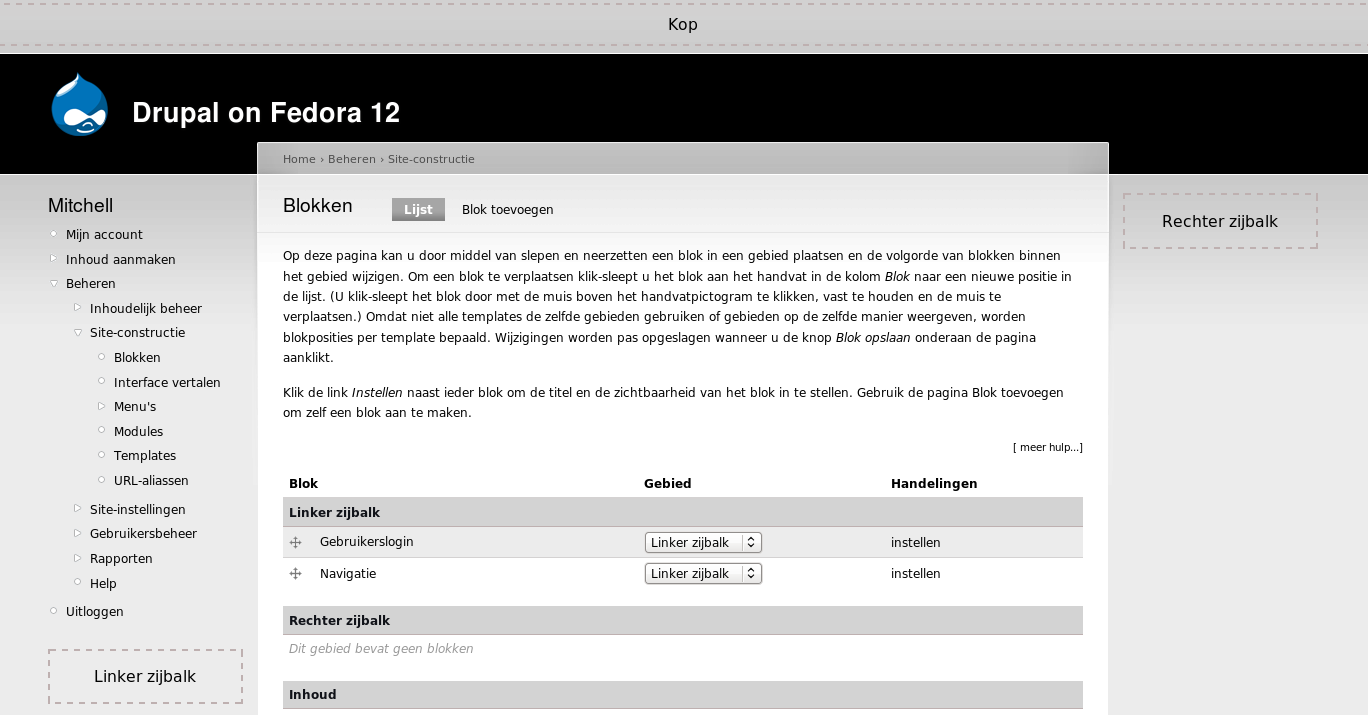
\includegraphics[scale=0.3,angle=0]{blokken-lijst}
   \caption{blokken-lijst.\label{white}}
 \end{figure}
 \subsection{Blok toevoegen} \index{blok toevoegen}
 Op deze pagina kunt u zelf een nieuw blok aanmaken. Nieuwe blokken zijn
 standaard uitgeschakeld en moeten op de pagina Blok beheren in een gebied geplaatst worden om te worden weergegeven.
 \begin{figure}[!h]
    \centering
   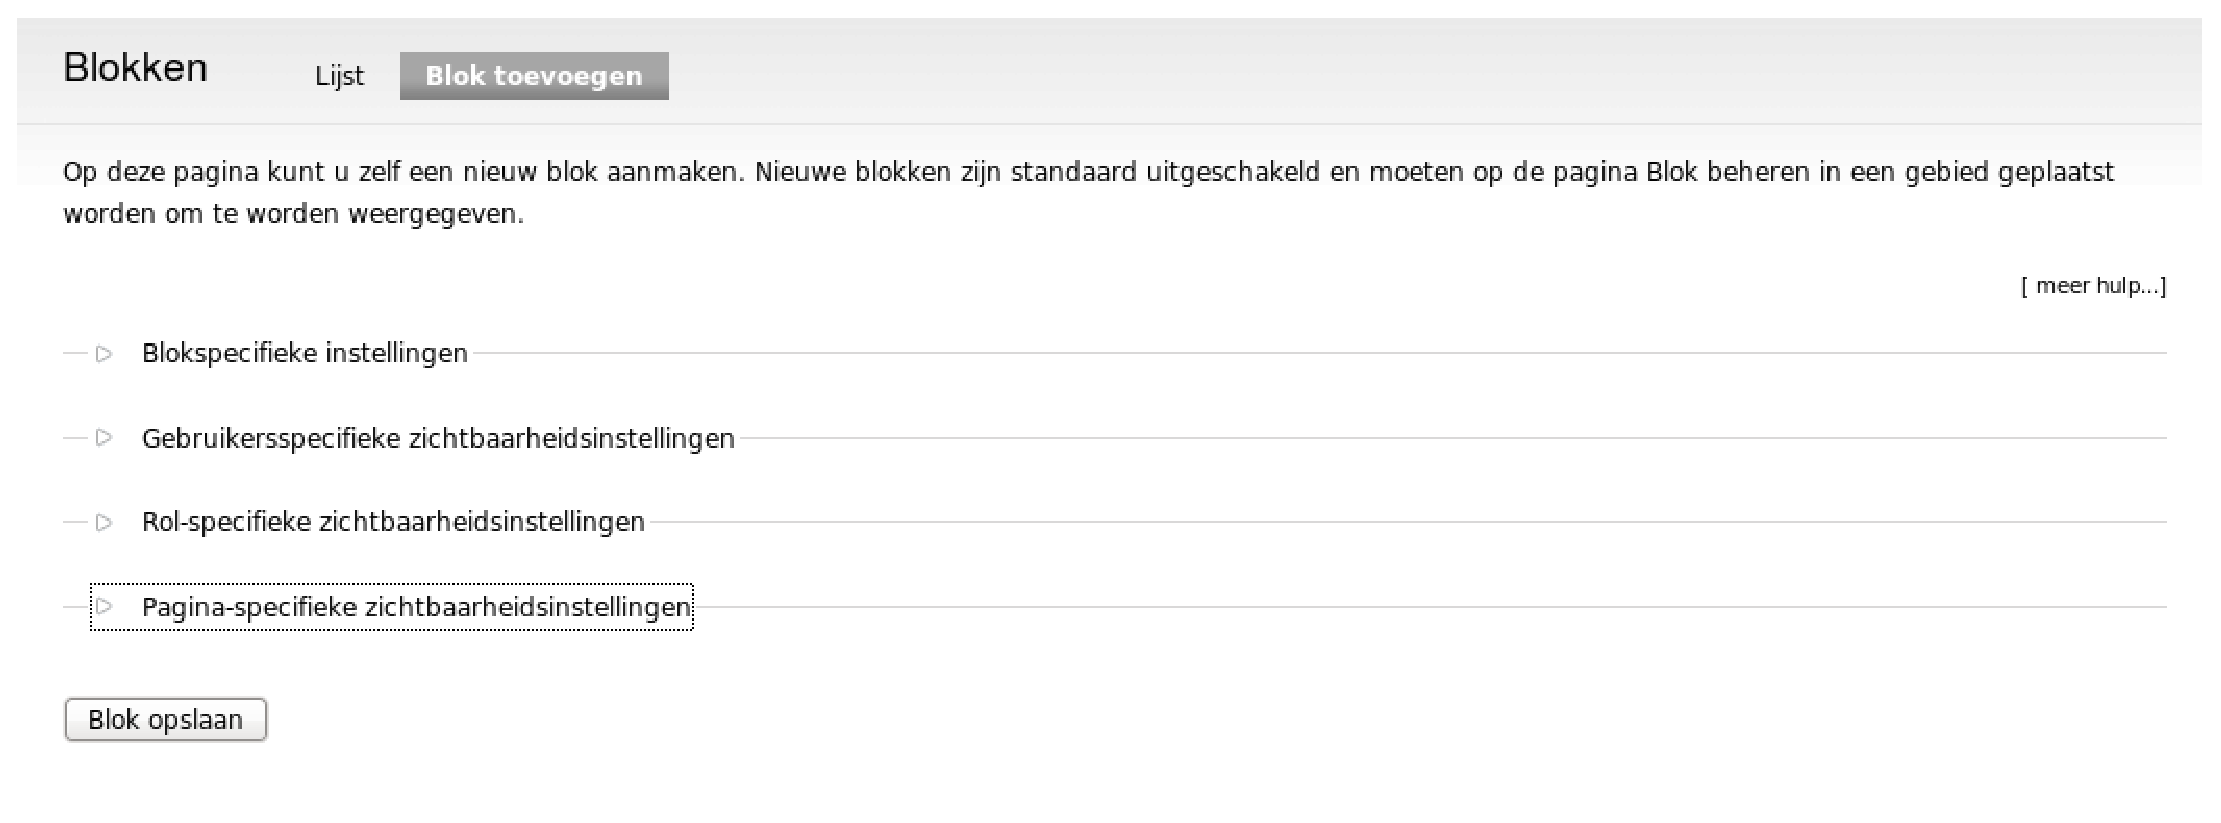
\includegraphics[scale=0.3,angle=0]{blok-toevoegen}
   \caption{blok-toevoegen.\label{white}}
 \end{figure}
\subsubsection{Blokspecifieke instellingen} \index{instellingen blok}
\begin{itemize}
\item Blokbeschrijving: Een korte beschrijving van het blok. Het wordt gebruikt op de blok overzichtspagina.
\item Bloktitel: De titel van een blok zoals getoond aan de gebruiker.
\item Blokinhoud: De inhoud van een blok zoals getoond aan de gebruiker.
\item Invoerformaat: Filtered HTML of Full HTML
\end{itemize}
 \begin{figure}[!h]
    \centering
   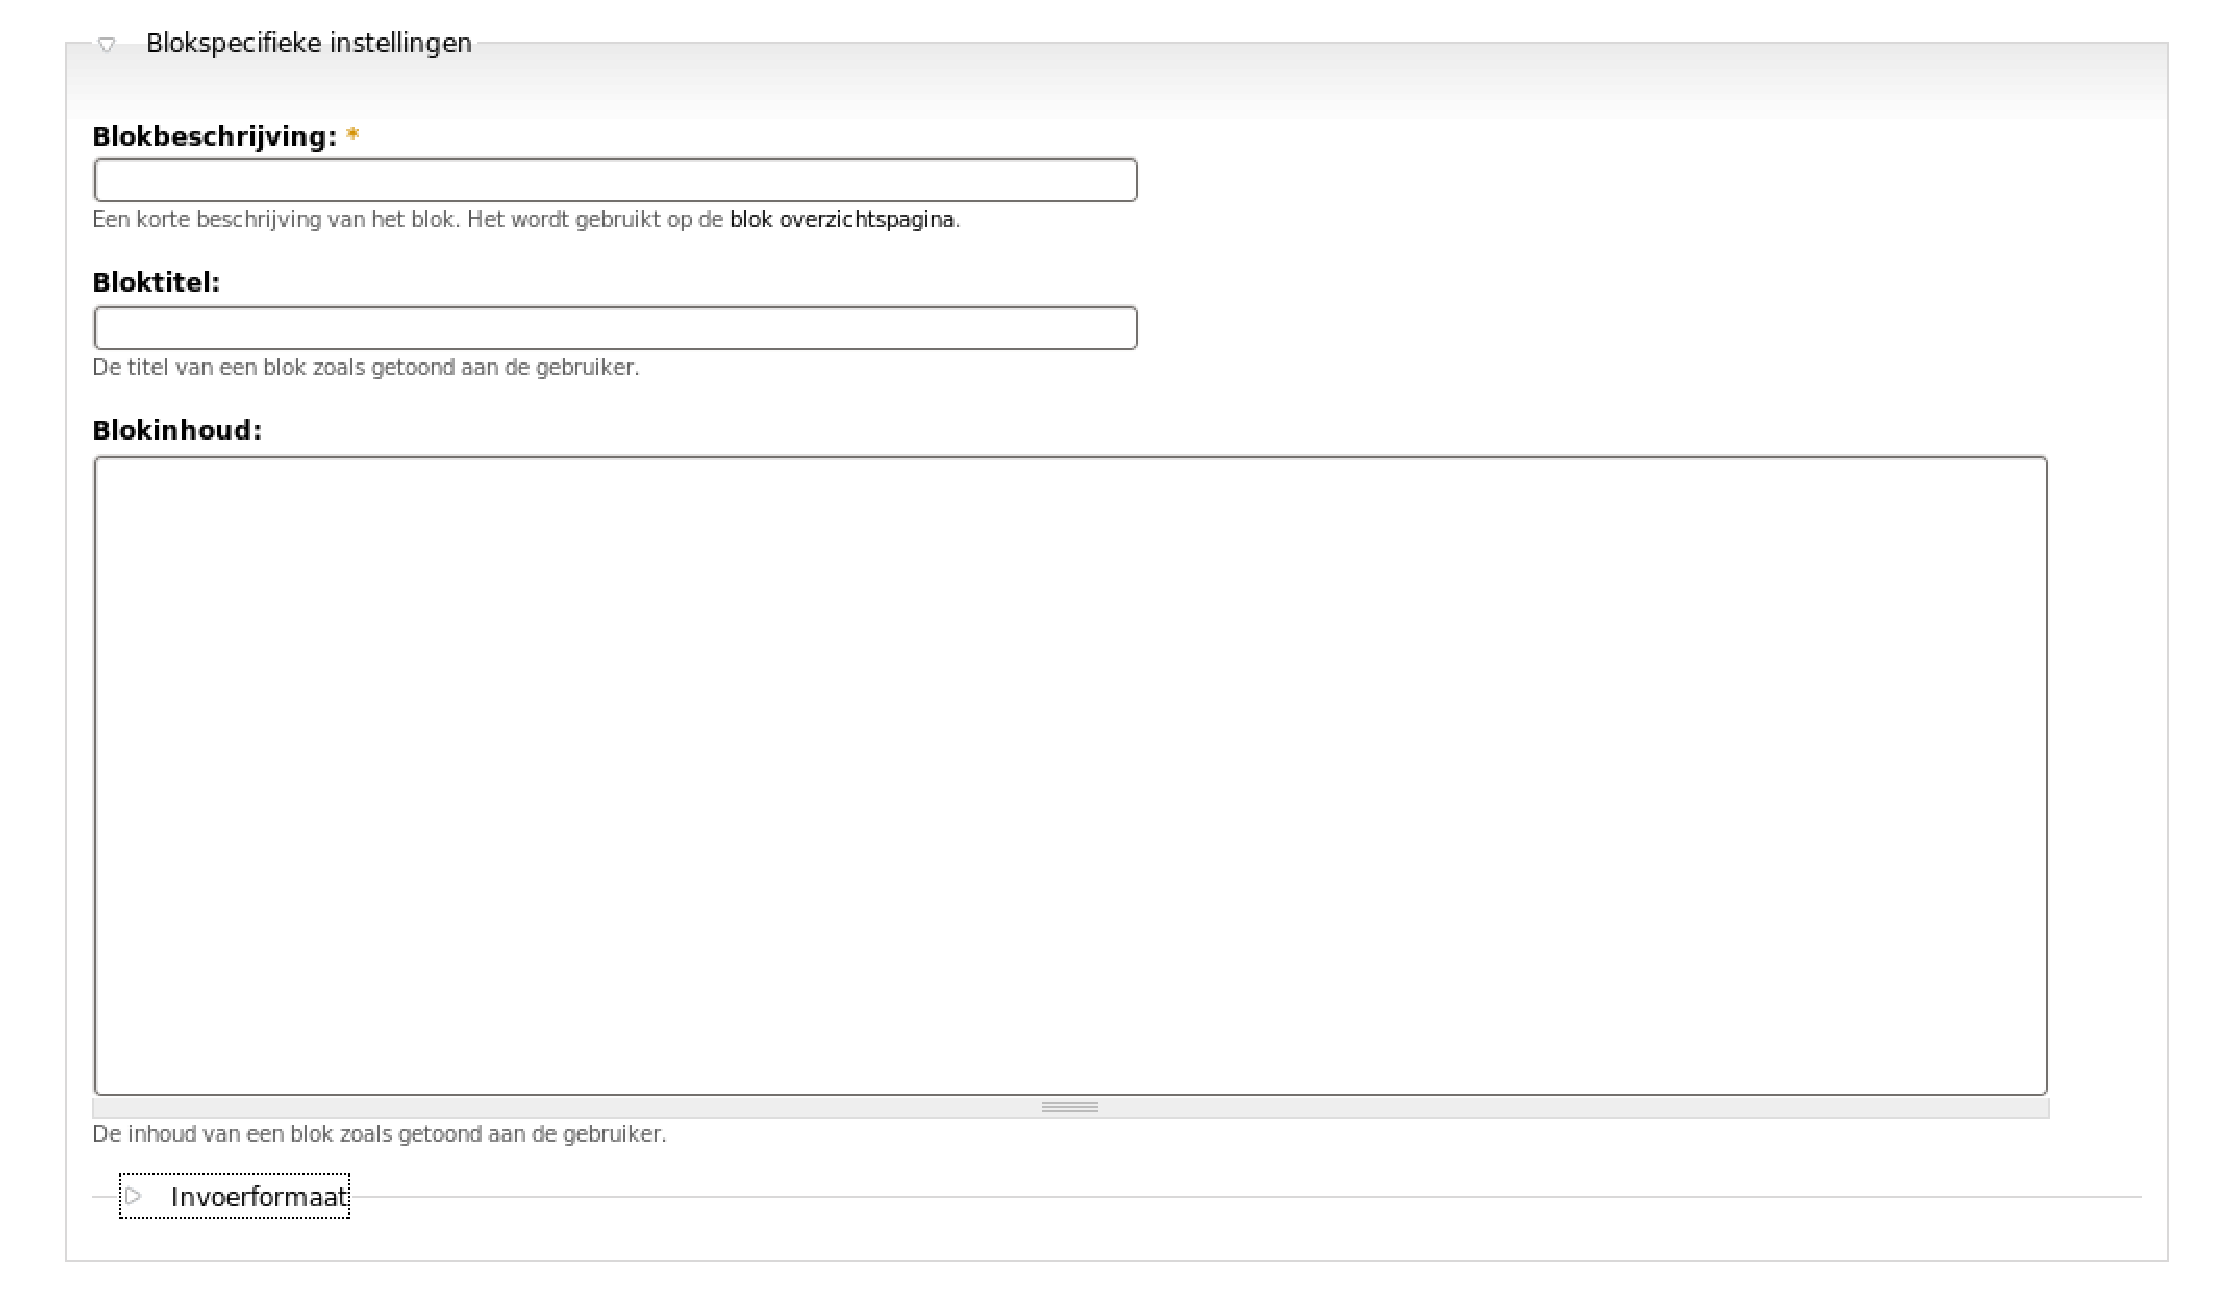
\includegraphics[scale=0.3,angle=0]{blok-specifieke-instellingen}
   \caption{blok-specifieke-instellingen.\label{white}}
 \end{figure}
\subsubsection{Gebruikersspecifieke zichtbaarheidsinstellingen}
\index{zichtbaarheidsinstellingen} Aangepaste zichtbaarheidsinstellingen: 
\begin{itemize}
\item Gebruikers kunnen niet kiezen of ze dit blok al dan niet willen zien.
\item Standaard dit blok weergeven. Individuele gebruikers kunnen ervoor kiezen het blok te verbergen.
\item Standaard dit blok verbergen. Individuele gebruikers kunnen ervoor kiezen het blok toch weer te geven.
\end{itemize}
Individuele gebruikers mogen de zichtbaarheid van dit blok in hun
gebruikersinstellingen aanpassen. 
\begin{figure}[!h]
    \centering
   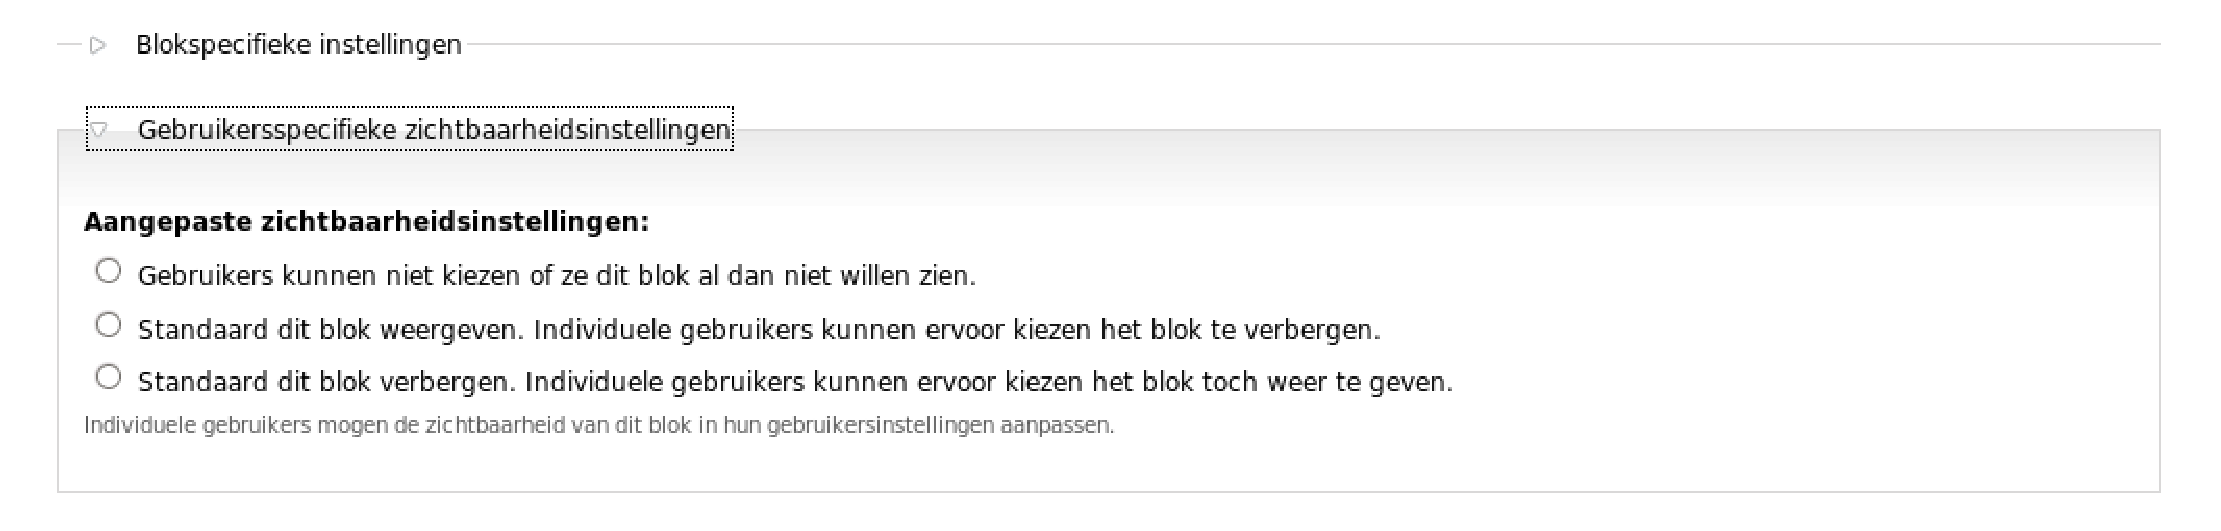
\includegraphics[scale=0.3,angle=0]{blok-gebruikers-specifieke}
   \caption{blok-gebruikers-specifieke.\label{white}}
 \end{figure} 
\subsubsection{Rol-specifieke zichtbaarheidsinstellingen}
Blok voor bepaalde rollen weergeven:  
\begin{itemize}
\item admin
\item anonymous user
\item authenticated user
\end{itemize}
Dit blok is alleen zichtbaar voor bepaalde rollen. Als u geen rollen selecteert is het blok voor alle gebruikers zichtbaar.
\begin{figure}[!h]
    \centering
   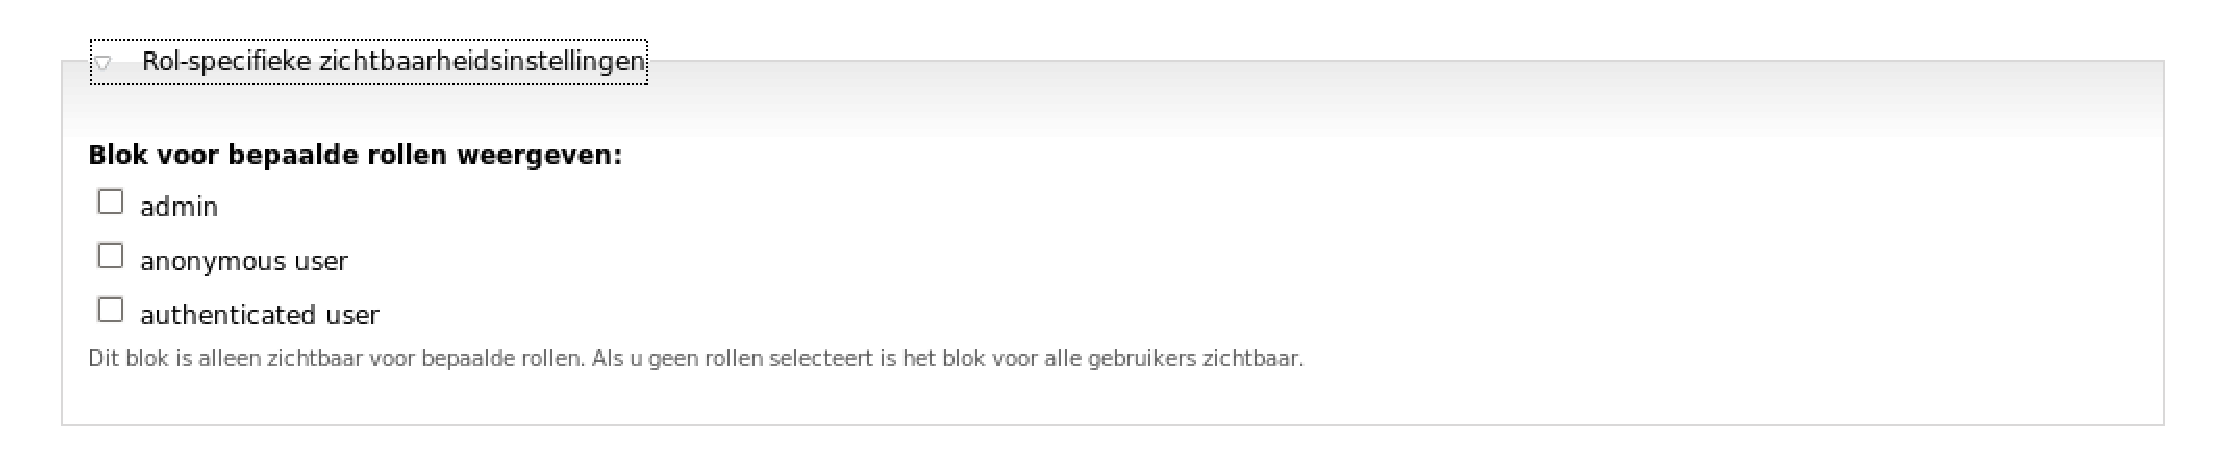
\includegraphics[scale=0.3,angle=0]{blok-rol-specifieke}
   \caption{blok-rol-specifieke.\label{white}}
 \end{figure} 
\subsubsection{Pagina-specifieke zichtbaarheidsinstellingen}
Blok op bepaalde pagina's weergeven:   
\begin{itemize}
\item Weergeven op elke pagina behalve op de vermelde pagina's.
\item Alleen weergeven op de vermelde pagina's.
\item Alleen weergeven wanneer de volgende PHP-code resulteert in TRUE. (PHP-mode, alleen voor experts).
\end{itemize}
Geef \'e\'en pagina per regel op, als Drupal-paden. Het '*'-teken is een
jokerteken. Voorbeeldpaden zijn 'blog' voor de blog-pagina en 'blog/*' voor elke
persoonlijke blog. '$<$front$>$' is de voorpagina. Als de PHP-modus wordt
gekozen geef dan de PHP-code op tussen $<$?php ?$>$. Merk op dat het uitvoeren
van incorrecte PHP-code uw Drupalsite defect kan maken. 
\begin{figure}[!h]
    \centering
   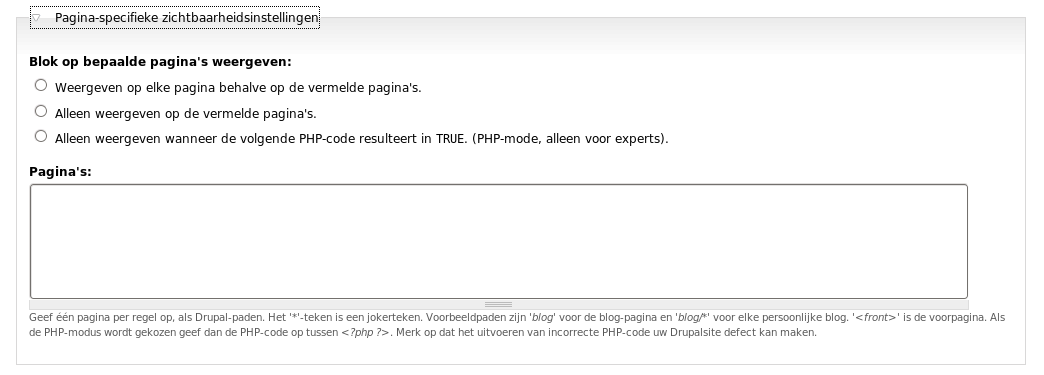
\includegraphics[scale=0.3,angle=0]{blok-pagina-specifieke}
   \caption{blok-pagina-specifieke.\label{white}}
 \end{figure} 



\section{Interface vertalen} \index{vertalen}
Deze pagina geeft een overzicht van vertaalbare tekenreeksen. Vertaalbare tekenreeksen 
worden weergegeven in zogenaamde 'tekstgroepen'. Modules kunnen extra tekstgroepen toevoegen 
die andere vertaalbare tekenreeksen bevatten. Omdat tekstgroepen een mogelijkheid bieden 
om tekenreeksen te groeperen, kunnen de tekstgroepen gebruikt worden om de vertaalinspanning 
te richten op bepaalde gebieden van de Drupal-interface.
\begin{figure}[!h]
    \centering
   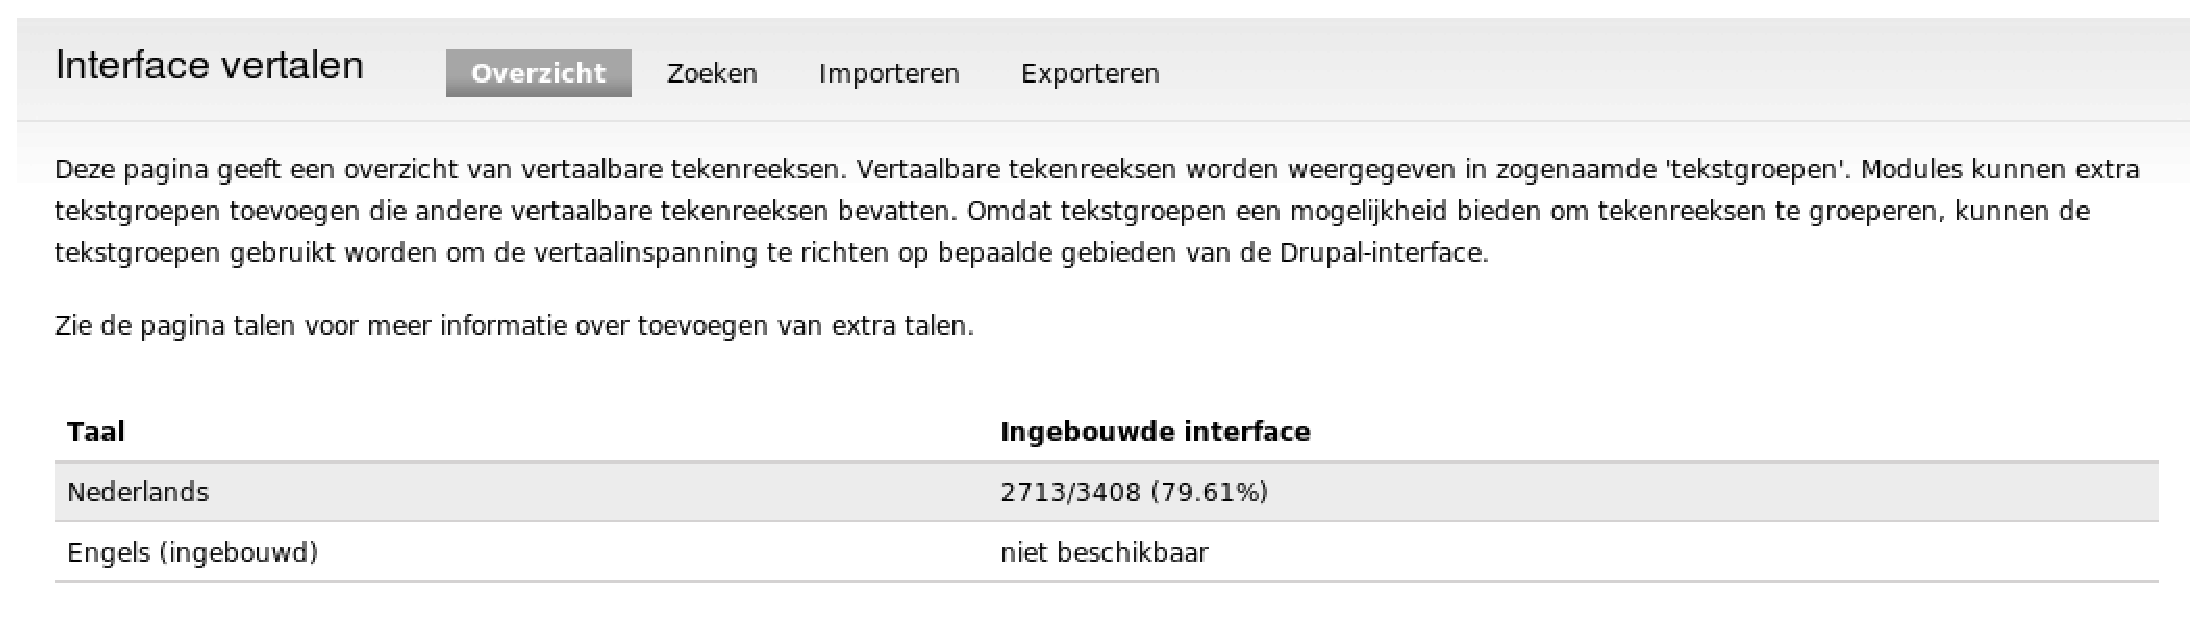
\includegraphics[scale=0.3,angle=0]{interfacevertalen-overzicht}
   \caption{interfacevertalen-overzicht.\label{white}}
 \end{figure}

\subsection{Interface vertalen - zoeken}
Op deze pagina kan een vertaler zoeken naar specifieke vertaalde en onvertaalde
tekenreeksen en vertalingen maken of bestaande vertalingen bijwerken. Merk op: 
voor het vertalen van vele tekenreeksen is het handiger om de tekenreeksen te 
exporteren en offline met een Gettext-editor te vertalen. 
Zoeken naar tekenreeksen kan beperkt worden tot een specifieke tekstgroep of een specifieke taal.
\begin{figure}[!h]
    \centering
   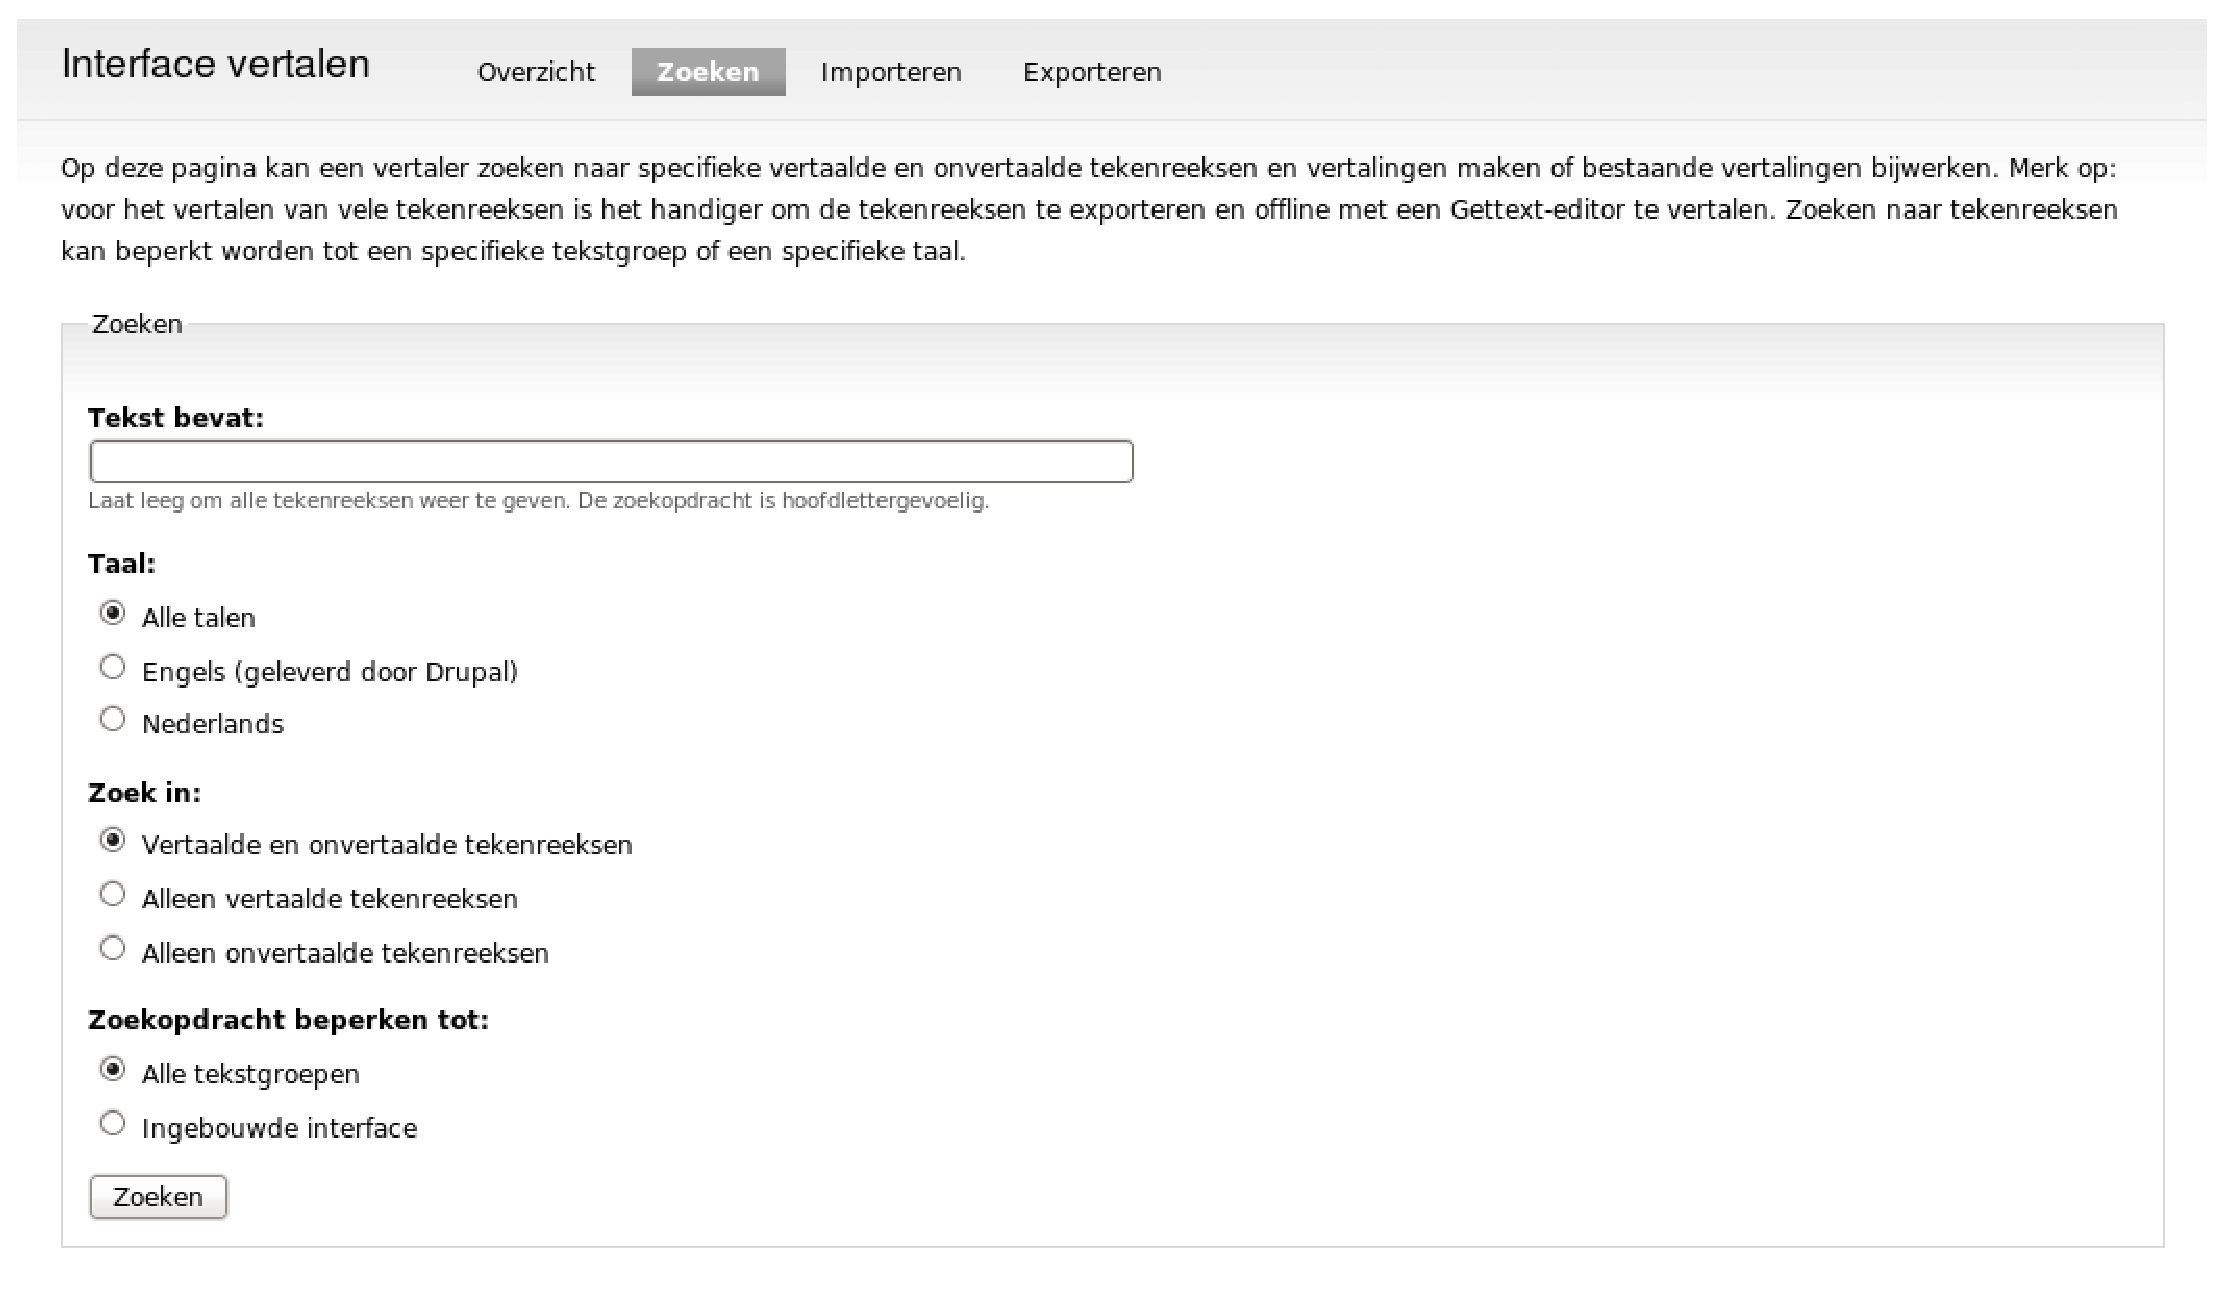
\includegraphics[scale=0.3,angle=0]{interfacevertalen-zoeken}
   \caption{interfacevertalen-zoeken.\label{white}}
 \end{figure}
 
\subsection{Importeren} \index{importeren}
Op deze pagina kunt u een vertaling als Gettext Portable Object (.po)-bestand importeren. 
Deze bestanden zijn gewoonlijk onderdeel van een vertaalpakket. Als een .po-bestand 
offline met een Gettext-editor wordt gewijzigd, kan u het bijgewerkte bestand op deze pagina 
importeren. Importeren van een .po-bestand kan enige tijd duren.
\\
Weet dat de .po-bestanden (indien aanwezig) automatisch ge\"importeerd worden
als een nieuwe module of template ingeschakeld wordt of als nieuwe talen worden toegevoegd. 
Omdat met deze pagina slechts \'e\'en .po-bestand tegelijkertijd ge\"importeerd
kan worden, kan het eenvoudiger zijn om een vertaalpakket te downloaden en in de Drupal-installatiemap 
uit te pakken en daarna de taal toe te voegen. Alle .po-bestanden in het vertaalpakket 
worden dan automatisch ge\"importeerd. Vertaalpakketten kunnen worden op de
Drupal Translations-pagina gedownload worden. \begin{figure}[!h]
    \centering
   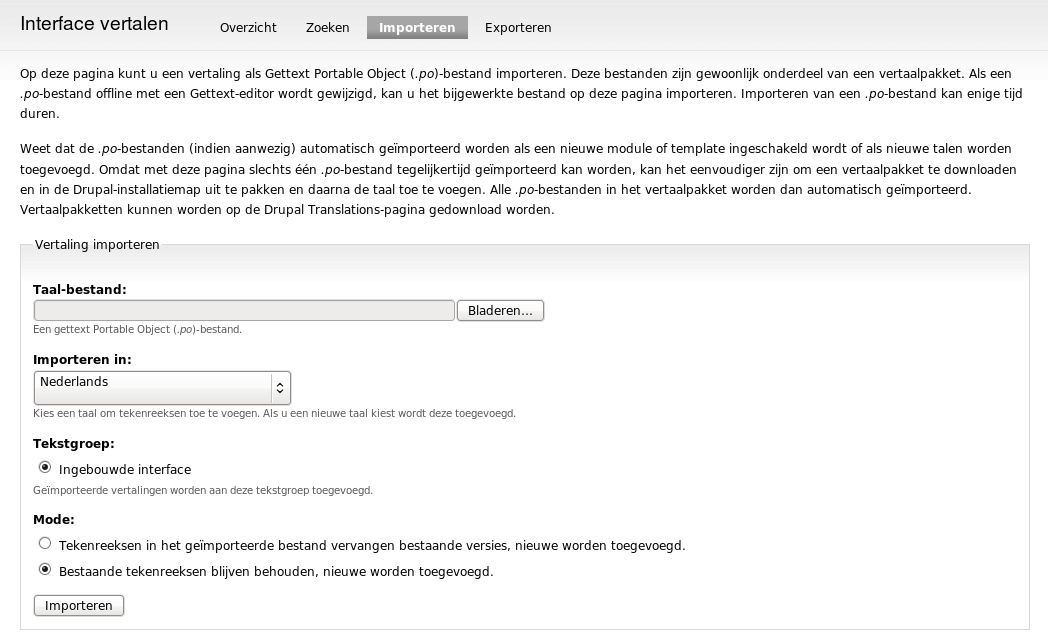
\includegraphics[scale=0.3,angle=0]{interfacevertalen-importeren}
   \caption{interfacevertalen-importeren.\label{white}}
 \end{figure}
 
\subsection{Exporteren} \index{exporteren} 
Op deze pagina kunt u vertaalde Drupal-tekenreeksen exporteren. De tekenreeksen kunnen in twee 
formaten als bestand ge\"exporteerd worden. Het Gettext Portable Object
(.po)-formaat, met daarin zowel de bron als de vertaalde tekenreeksen, of het Gettext Portable Object Template (.pot)-formaat, 
met daarin alleen de bron-tekenreeksen. Het .po-formaat wordt gebruikt om vertaling met anderen te delen, 
het .pot-formaat om met een Gettext-editor een nieuwe vertaling te maken.
\begin{figure}[!h]
    \centering
   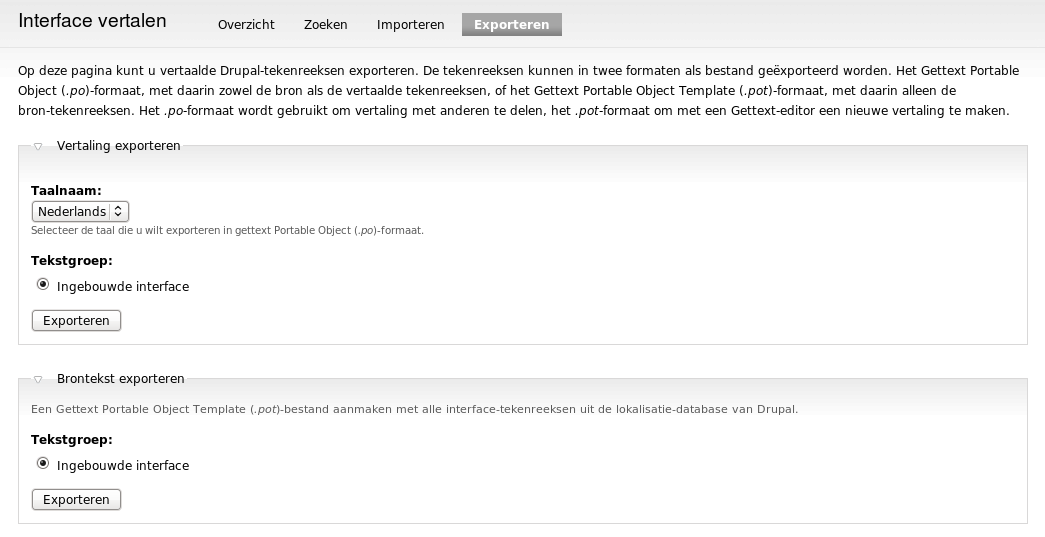
\includegraphics[scale=0.3,angle=0]{interfacevertalen-exporteren}
   \caption{interfacevertalen-exporteren.\label{white}}
 \end{figure}

\section{Menu's} \index{menu}
Navigatiemenu, \index{navigatiemenu} primaire \index{primaire links} en
secundaire links \index{secundaire links} beheren, menu-onderdelen hernoemen en
menu's reorganiseren.

\subsection{Menu-module} \index{menu-module}
De Menu-module biedt de mogelijkheid om het Drupal menu-systeem te beheren en in te stellen. 
Menu's zijn een verzameling van links (menu-onderdelen) die worden gebruikt om binnen de 
website te navigeren en worden met behulp van Drupal-blokken binnen een pagina gepositioneerd 
en weergegeven. Standaard worden tijdens installatie drie menu's aangemaakt: Navigatie, Primaire links en Secundaire links. 
Het Navigatiemenu bevat de menu-onderdelen die nodig zijn om de website te beheren en wordt vaak in de linker of rechter 
zijbalk weergegeven. De meeste Drupal-templates ondersteunen Primaire links en Secundaire links en geven deze menu's in 
kop of voet van de pagina weer. Standaard bevatten Primaire links en Secundaire links geen menu-onderdelen, maar deze 
kunnen door de beheerder met website-specifieke menu-onderdelen worden gevuld.
\\
De pagina menu's bevat alle menu's die op de site beschikbaar zijn. Selecteer een menu om menu-onderdelen toe 
te voegen, te wijzingen of de volgorde van menu-onderdelen binnen het menu te veranderen. Op de pagina menu 
toevoegen kunt u een menu toevoegen (Op de pagina Blokken beheren kunt u het blok dat dit menu bevat inschakelen).

\subsection{Menu's weergeven}
Menu's zijn een verzameling van links (menu-onderdelen) die worden gebruikt om
binnen de website te navigeren. Hier onder vindt u alle menu's die op de site beschikbaar zijn. 
Selecteer een menu uit de lijst om de bijbehorende menu-onderdelen te beheren.
\begin{figure}[!h]
    \centering
   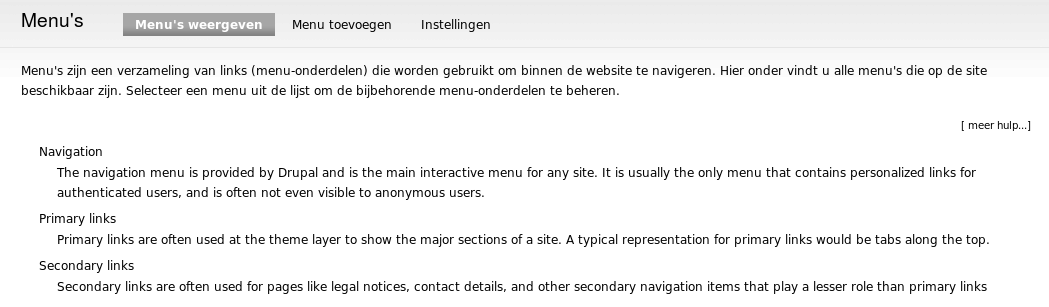
\includegraphics[scale=0.3,angle=0]{menu-weergeven}
   \caption{menu-weergeven.\label{white}}
 \end{figure}

\subsection{Menu toevoegen}
Geef de naam op voor een nieuw menu. Vergeet niet het nieuw aangemaakte blok in
de pagina blokbeheer in te schakelen.
\begin{figure}[!h]
    \centering
   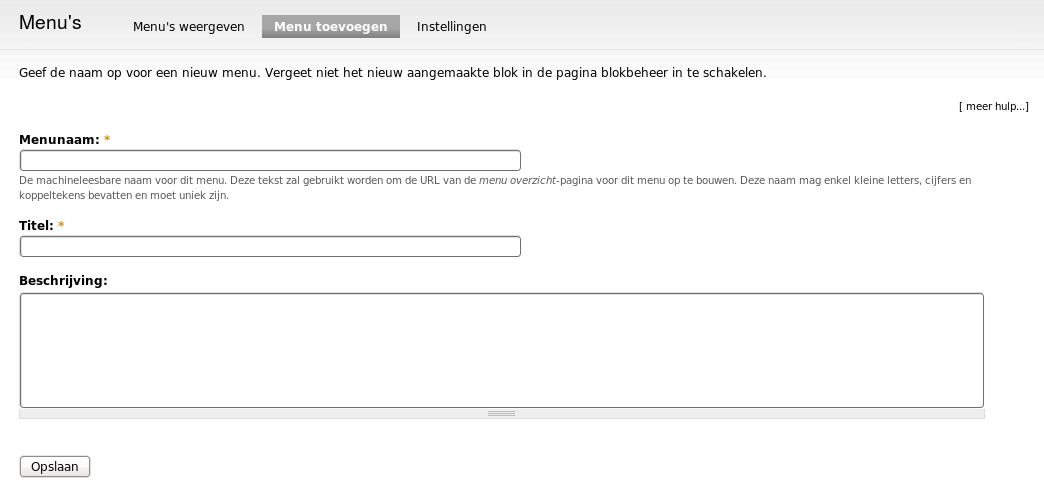
\includegraphics[scale=0.3,angle=0]{menu-toevoegen}
   \caption{menu-toevoegen.\label{white}}
 \end{figure}

\subsection{Instellingen}
De Menu-module maakt het mogelijk om in het node-invoer- en bewerkingsformulier
een menu-link naar de node aan te maken. De volgende optie bepaalt het standaardmenu waaraan een nieuwe link zal worden toegevoegd. 
\begin{figure}[!h]
    \centering
   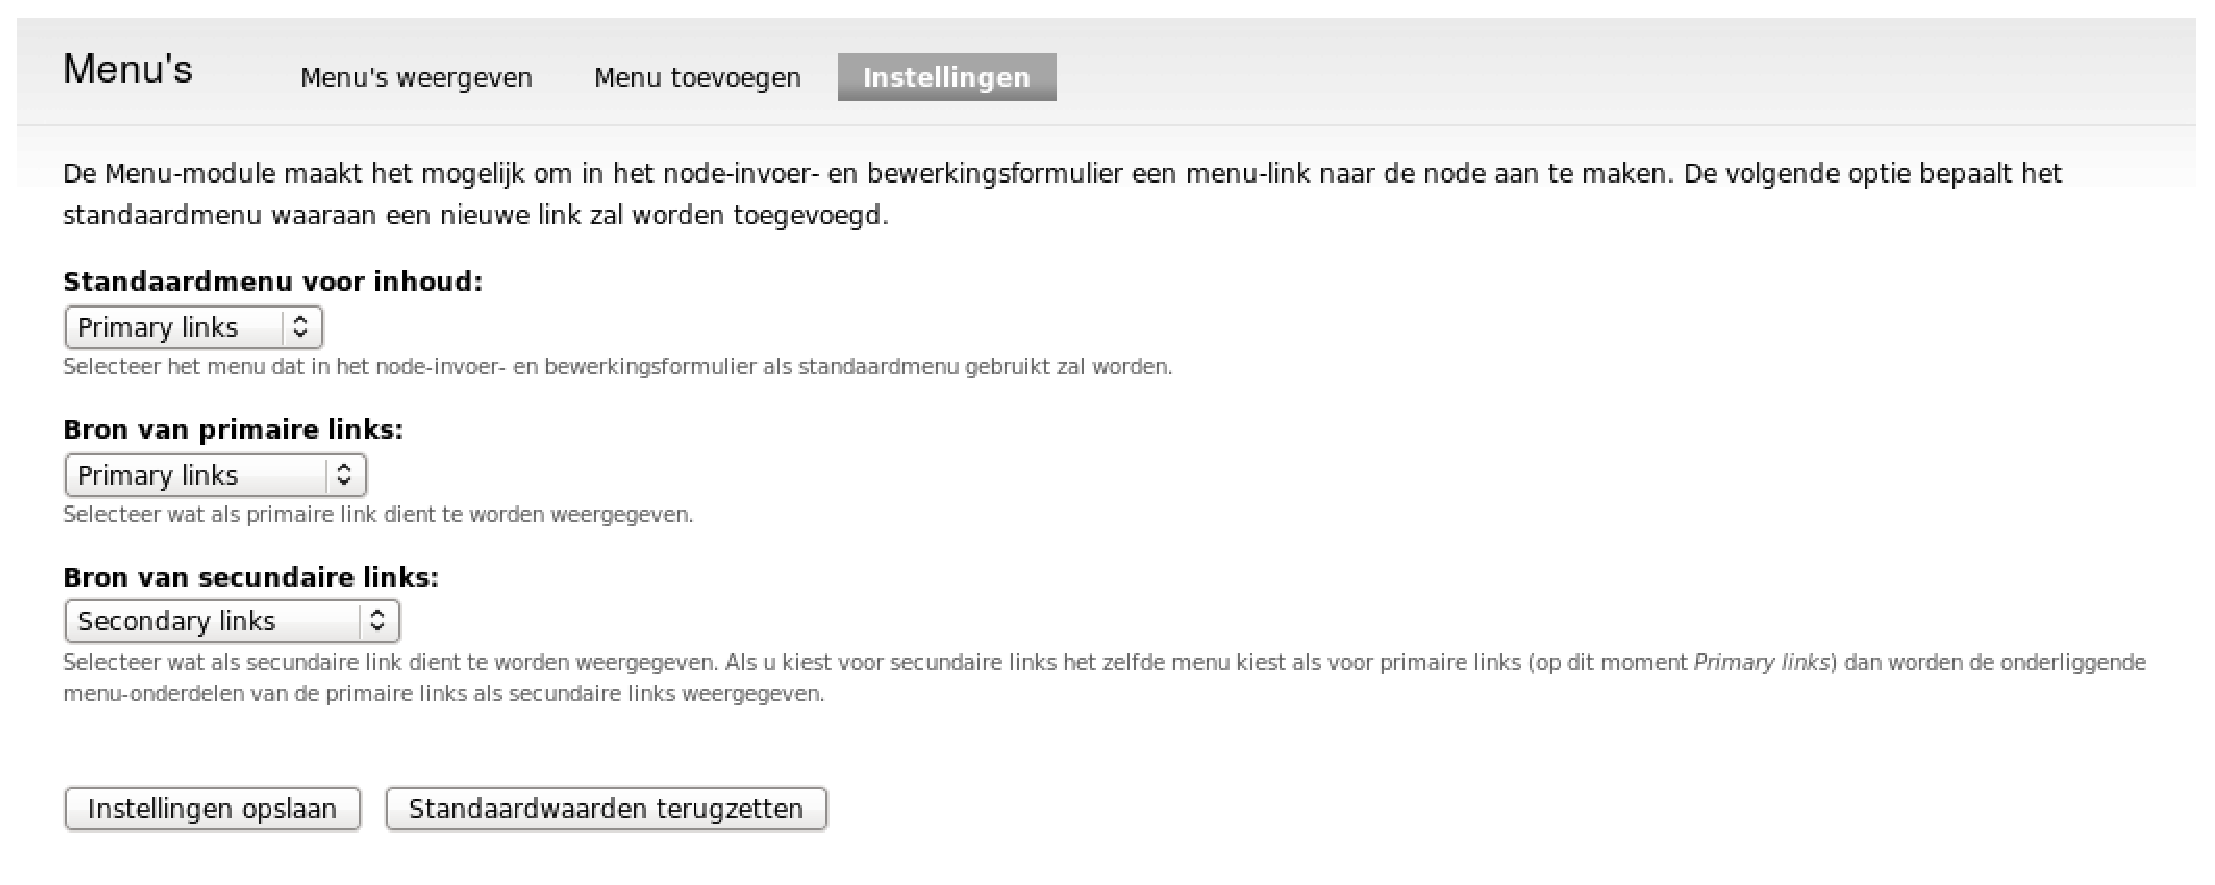
\includegraphics[scale=0.3,angle=0]{menu-instellingen-01}
   \caption{menu-instellingen-01.\label{white}}
 \end{figure}

\subsection{Navigation}
Om menu-onderdelen te verplaatsen klik-sleept u deze aan het handvat in de kolom
Menu-item naar een nieuwe positie in de lijst. (U klik-sleept het blok door met de muis boven het handvatpictogram te klikken, 
vast te houden en de muis te verplaatsen.) Wijzigingen worden pas opgeslagen wanneer u de knop Opslaan onderaan de pagina aanklikt.
\begin{figure}[!h]
    \centering
   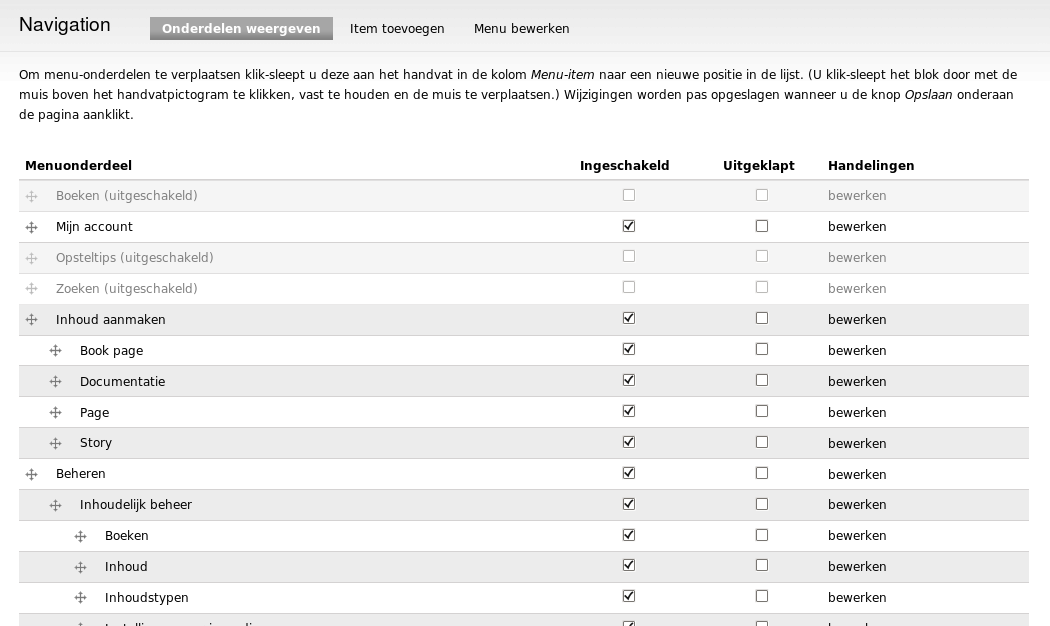
\includegraphics[scale=0.3,angle=0]{nav-onderdelen-weergeven}
   \caption{nav-onderdelen-weergeven.\label{white}}
 \end{figure}
% \subsubsection{item toevoegen}
% \begin{figure}[!h]
%     \centering
%    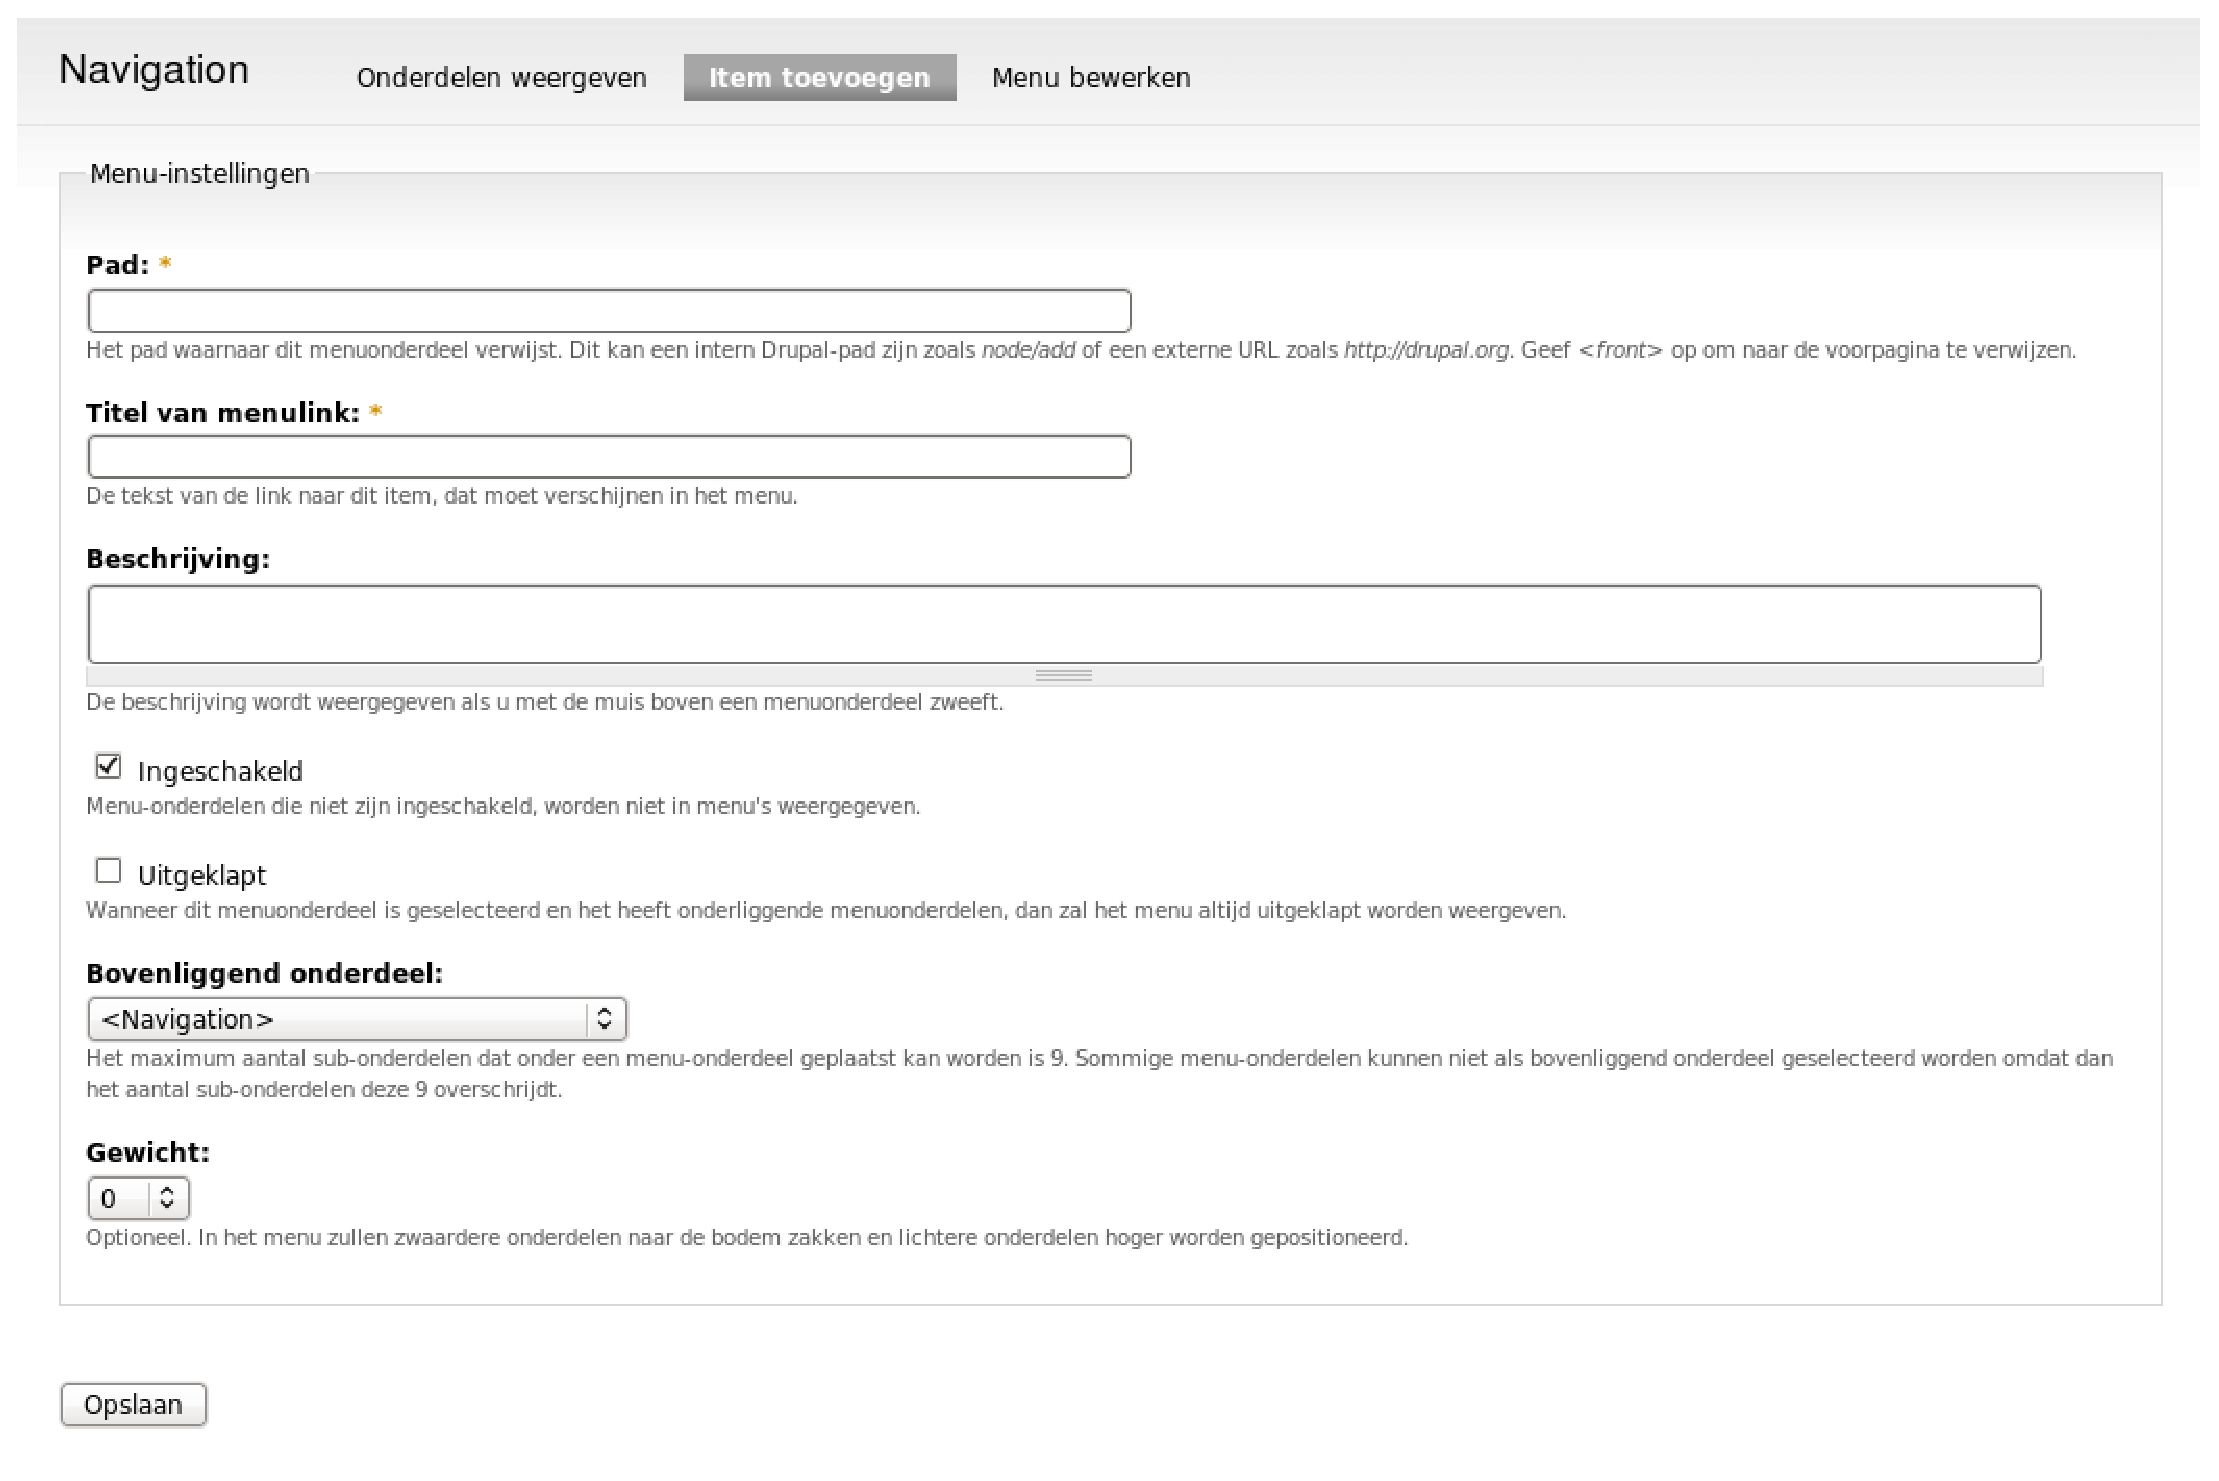
\includegraphics[scale=0.3,angle=0]{nav-item-toevoegen}
%    \caption{nav-item-toevoegen.\label{white}}
%  \end{figure}
%  \subsubsection{Menu bewerken}
%  \begin{figure}[!h]
%     \centering
%    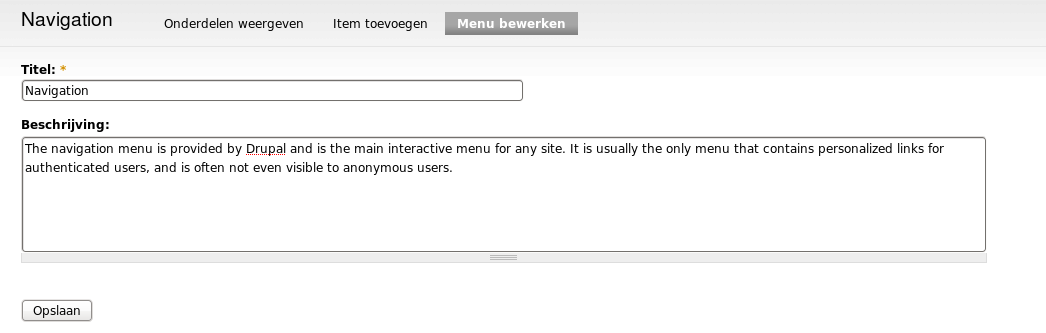
\includegraphics[scale=0.3,angle=0]{nav-menu-bewerken}
%    \caption{nav-menu-bewerken.\label{white}}
%  \end{figure}



\section{Modules} \index{modules}
Modules zijn plugins \index{plugins} voor Drupal die de kernfunctionaliteit
uitbreiden.
\subsection{Module lijst}
Hier kunt u de ingeschakelde 
modules kiezen. Klik in het navigatiemenu op de naam van de module voor de betreffende instellingenpagina. 
Als een module eenmaal is ingeschakeld kunnen nieuwe toegangsrechten beschikbaar zijn. 
Met behulp van de Throttle-module \index{throttle-module} kunnen modules
automatisch tijdelijk worden uitgeschakeld om de belasting van de server te verminderen op momenten dat de site extreem druk wordt bezocht.
\\
Het is belangrijk om update.php uit te voeren nadat een nieuwere versie van een
module is ge\"installeerd.
\\
U kunt alle beheertaken van een bepaalde module vinden op de pagina beheer per module.
\begin{figure}[!h]
    \centering
   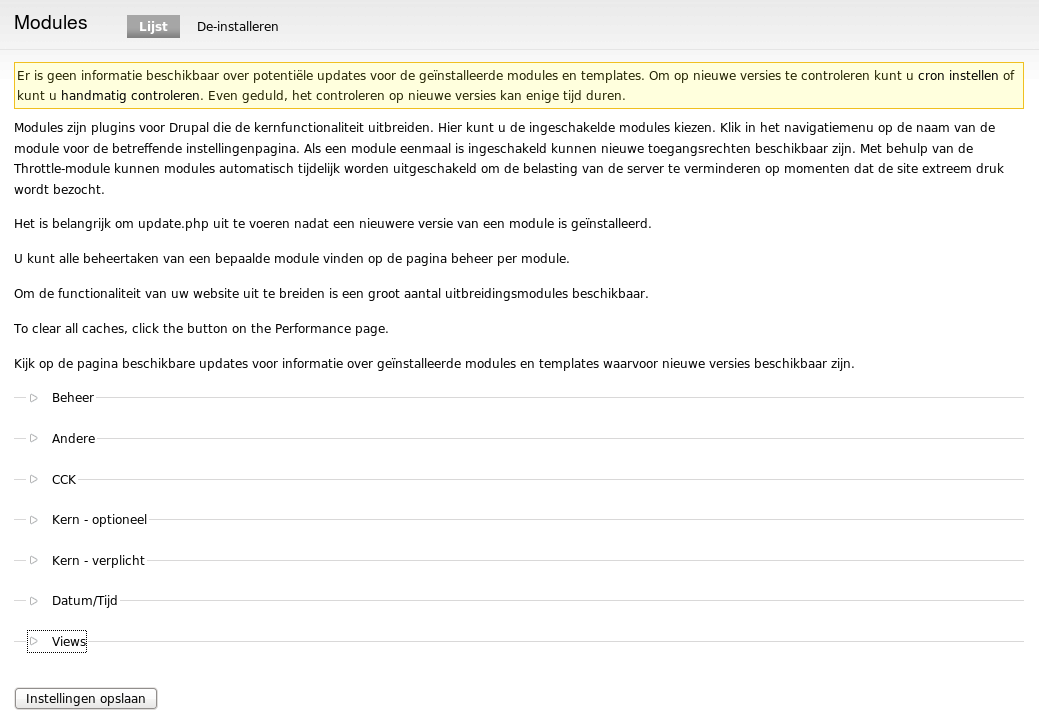
\includegraphics[scale=0.3,angle=0]{modules-lijst}
   \caption{modules-lijst.\label{white}}
 \end{figure}
 Om de functionaliteit van uw website uit te breiden is een groot aantal
 uitbreidingsmodules beschikbaar.
 
 
\subsection{Modules de-installeren} \index{de-installeren modules}
Het de-installatie proces verwijdert alle gegevens aan een module gerelateerde
gegevens. Schakel een module eerst uit, alvorens deze te de-installeren. De-installatie wordt niet door alle modules ondersteund.
\begin{figure}[!h]
    \centering
   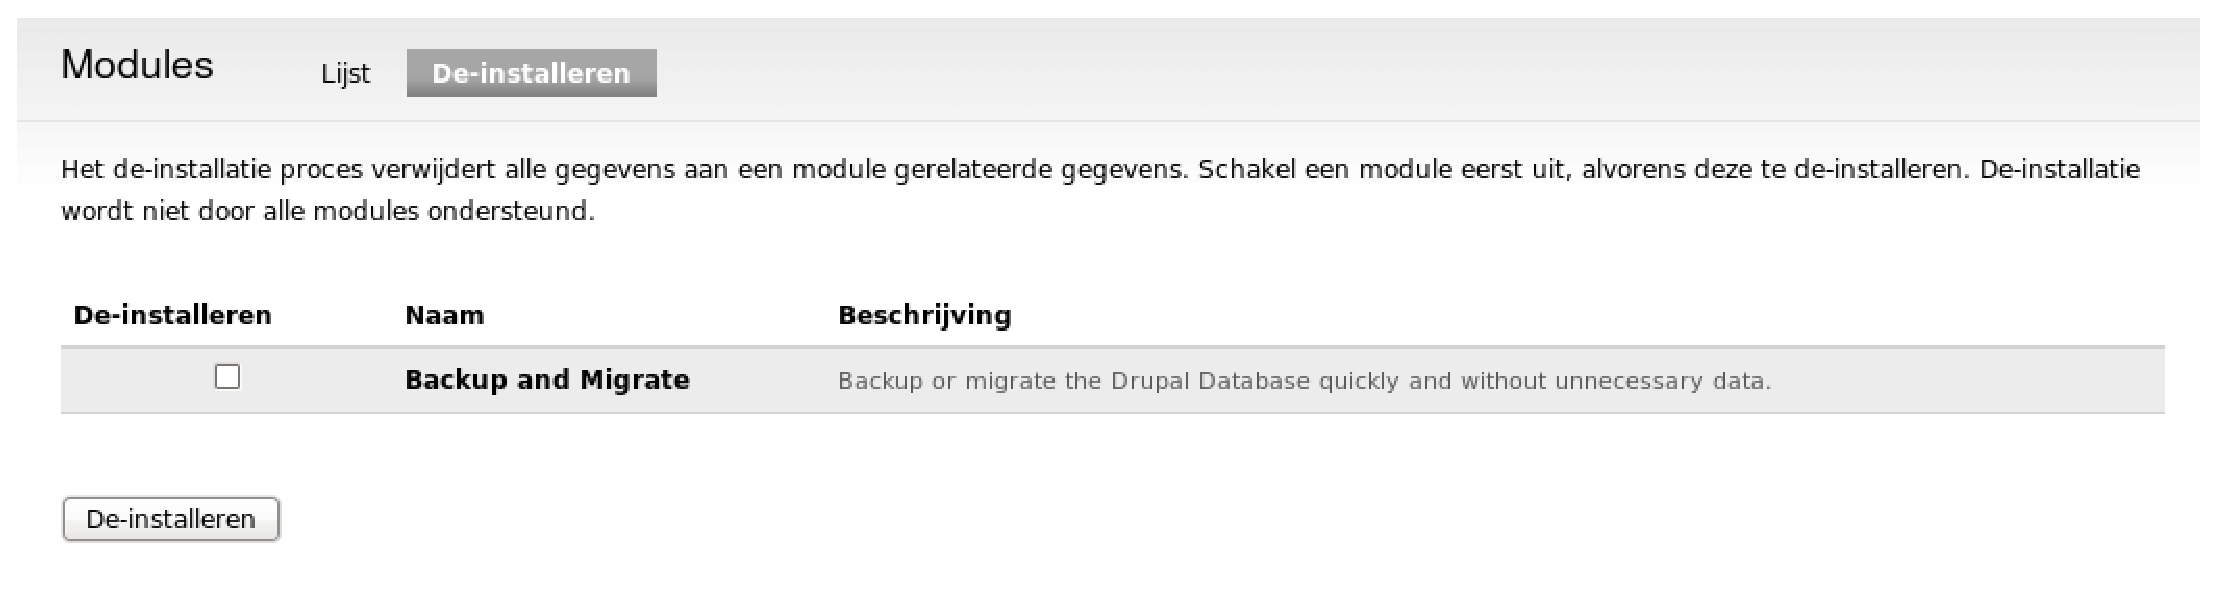
\includegraphics[scale=0.3,angle=0]{modules-deinstalleren}
   \caption{modules-deinstalleren.\label{white}}
 \end{figure}

\section{Templates} \index{templates}
De template voor de weergave van de site bepalen of deze keuze aan de gebruikers
laten. Om het uiterlijk van uw website te veranderen zijn er diverse
uitbreidingstemplates beschikbaar.

\subsection{Templates lijst}
Selecteer de templates die voor uw gebruikers beschikbaar zijn en stel een
standaard template in. Klik voor algemene weergave-instellingen op de Link 'instellen' hierboven. 
Klik op de link voor het betreffende template waarvoor u deze instellingen wilt wijzigen. 
Let er op dat verschillende templates verschillende regionen voor weergave van inhoud kunnen hebben; 
voor consistentie in de presentatie kunt u het best slechts \'e\'en template
inschakelen. \begin{figure}[!h]
    \centering
   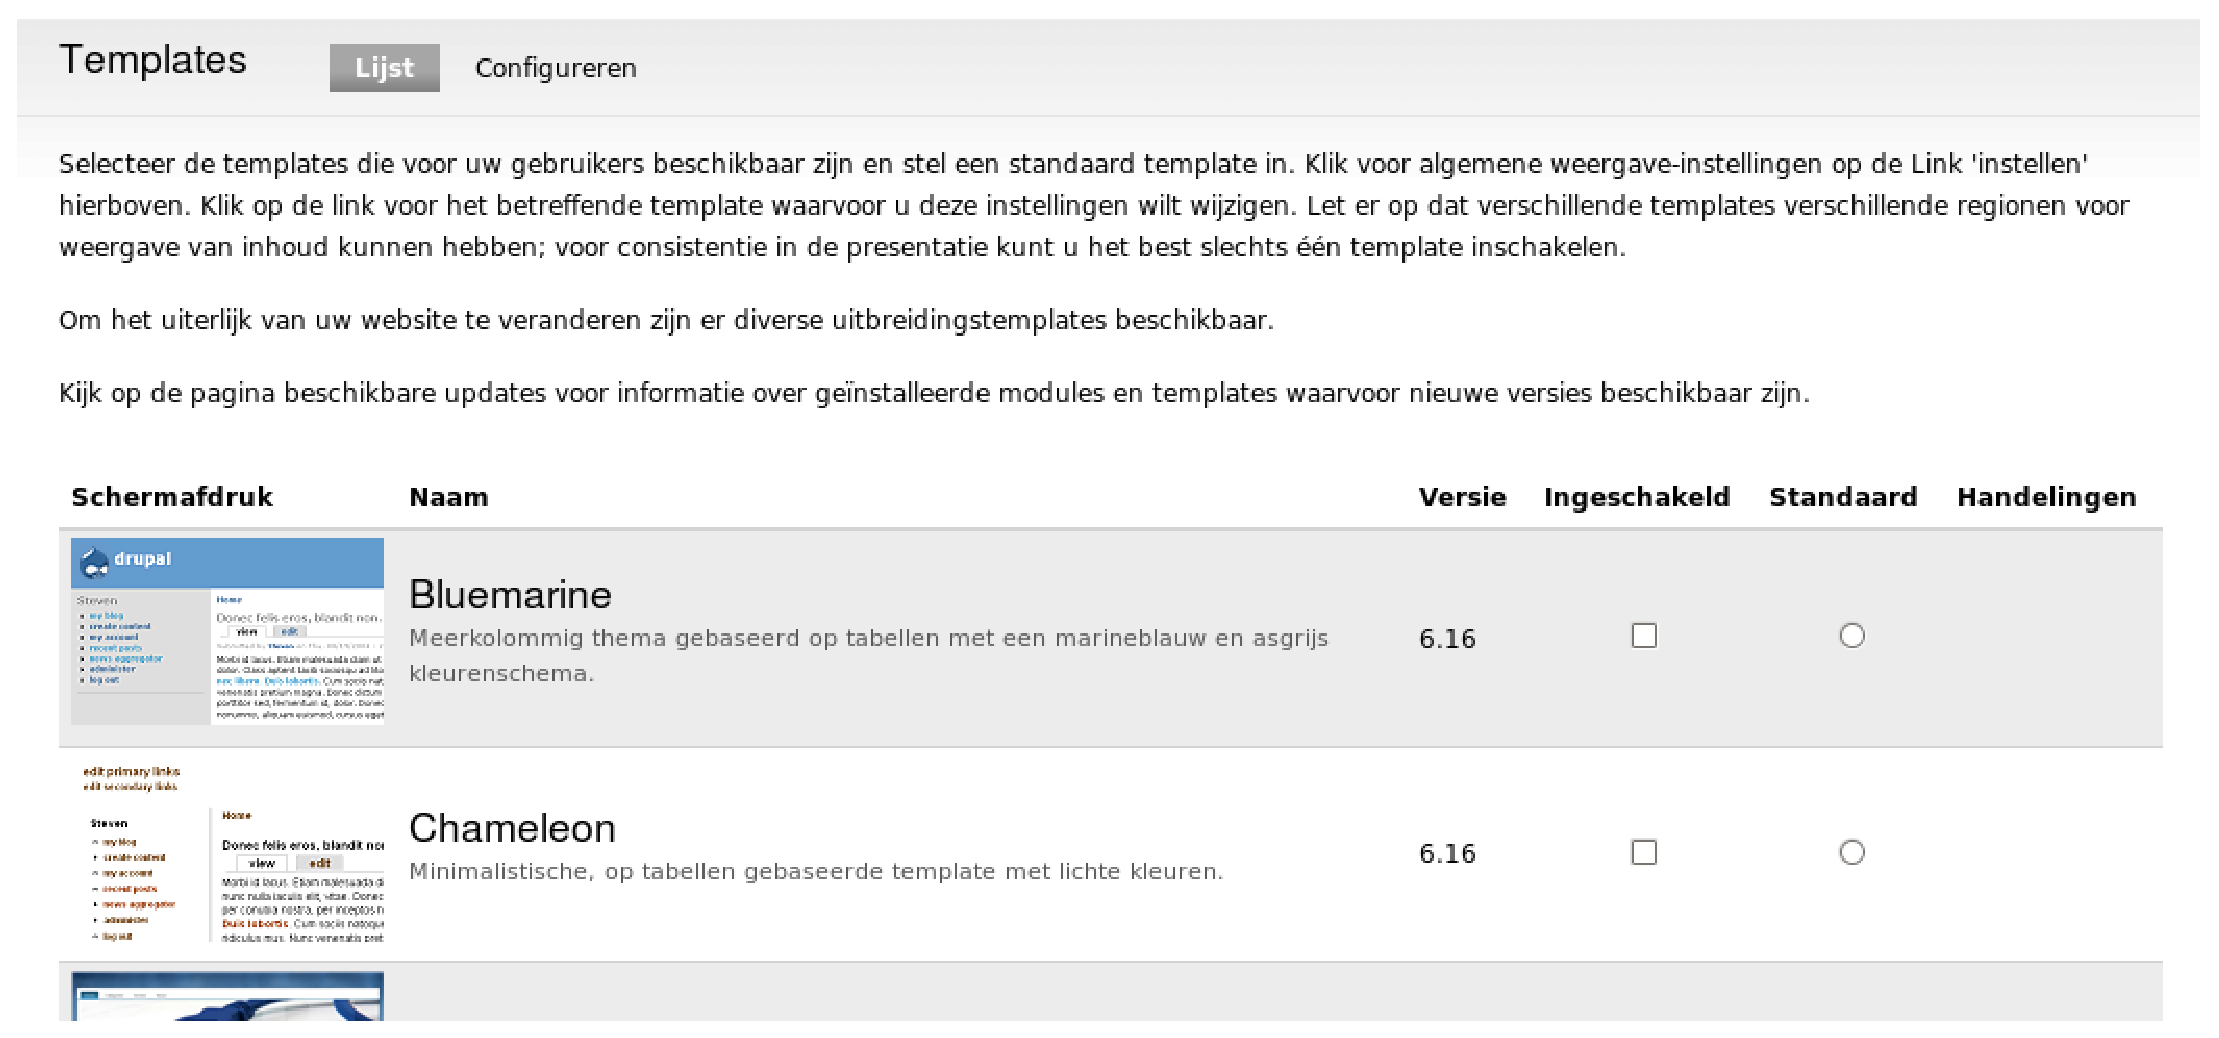
\includegraphics[scale=0.3,angle=0]{templates-lijst}
   \caption{templates-lijst.\label{white}}
 \end{figure}
 
 \subsection{Configureren globale instellingen} \index{globale instellingen}
 Deze opties sturen de standaard weergave-instellingen voor uw volledige website
 voor alle templates. Tenzij deze teniet gedaan worden door een specifieke template, zullen deze instellingen gebruikt worden.
 \begin{figure}[!h]
    \centering
   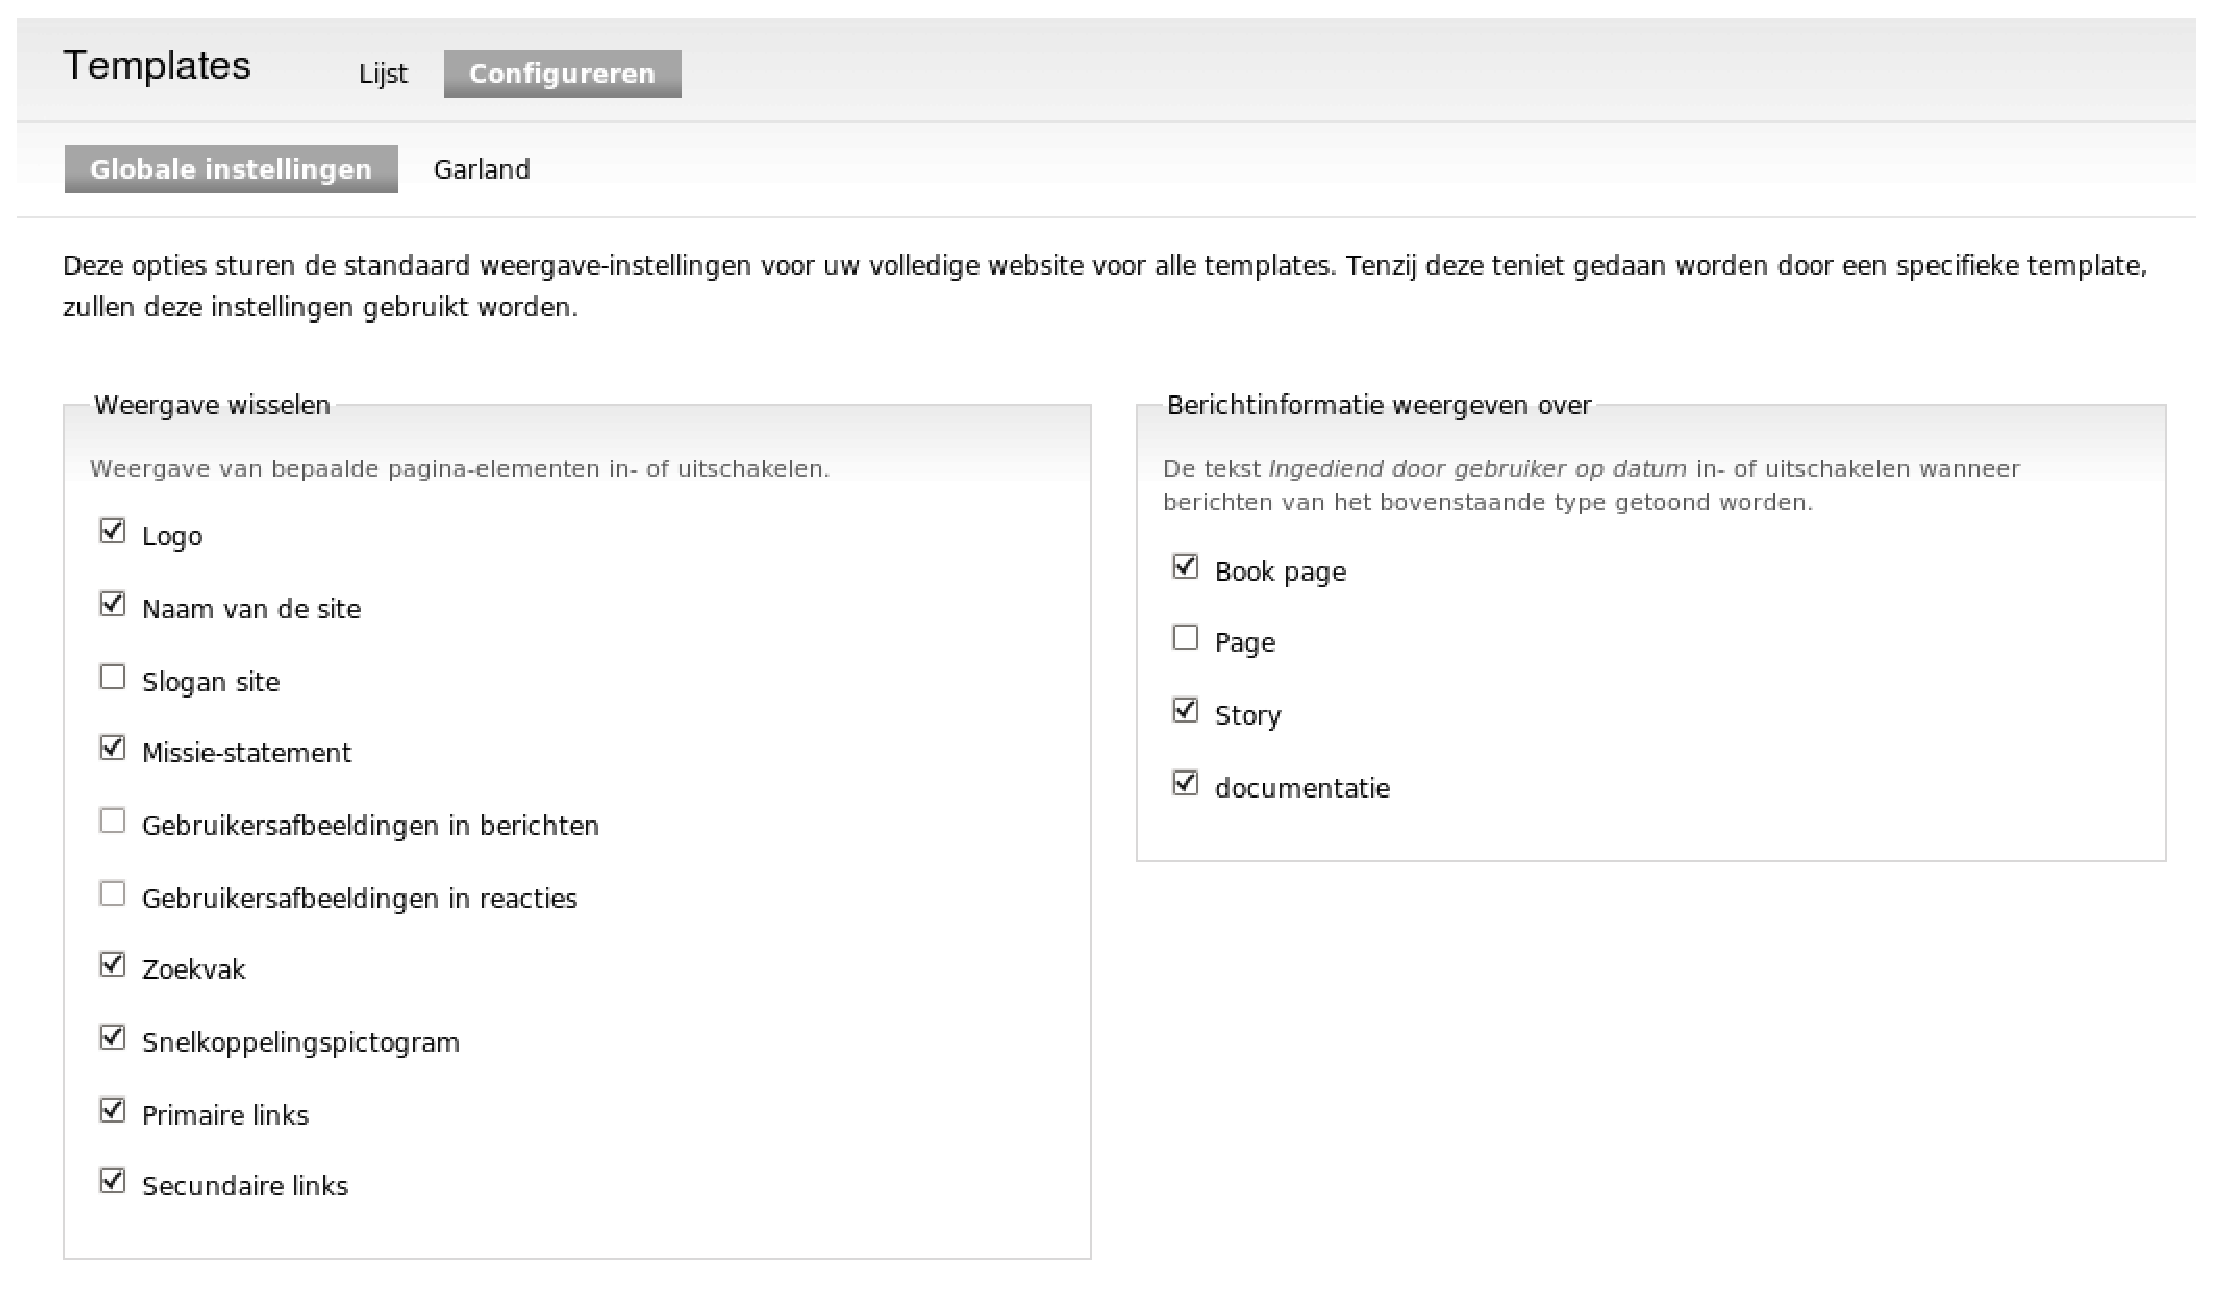
\includegraphics[scale=0.3,angle=0]{templates-globale-instellingen}
   \caption{templates-globale-instellingen.\label{white}}
 \end{figure}
 
\subsection{Configureren specifieke template instellingen} 
Deze opties bepalen de weergave-instellingen van de garland-template. Wanneer uw
website met deze template wordt weergegeven, zullen deze instellingen gebruikt worden. Door op "Standaardwaarden terugzetten" te klikken, 
kunt u de globale instellingen voor deze template gebruiken.
 \begin{figure}[!h]
    \centering
   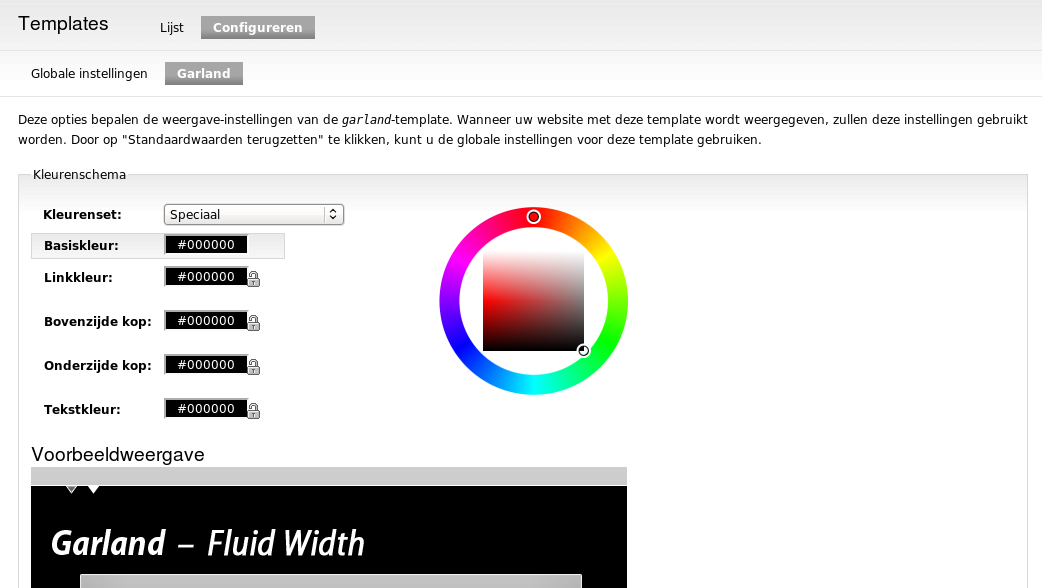
\includegraphics[scale=0.3,angle=0]{templates-garland}
   \caption{templates-garland.\label{white}}
 \end{figure}
 
\section{URL-aliassen} \index{aliassen}
De URL-paden van de site met behulp van aliassen wijzigen.

\subsection{URL-aliassen lijst}
Drupal biedt volledige controle over URL's door het gebruik van aliassen. 
Deze voorziening wordt meestal gebruikt om URL's makkelijker leesbaar te maken 
of eenvoudiger te herinneren. Zo kan men bijvoorbeeld het systeempad 'node/1' verbinden aan 'over-ons' en 
zo de URL een betekenis geven. Elk systeempad kan aan meerdere aliassen gekoppeld zijn.
 \begin{figure}[!h]
    \centering
   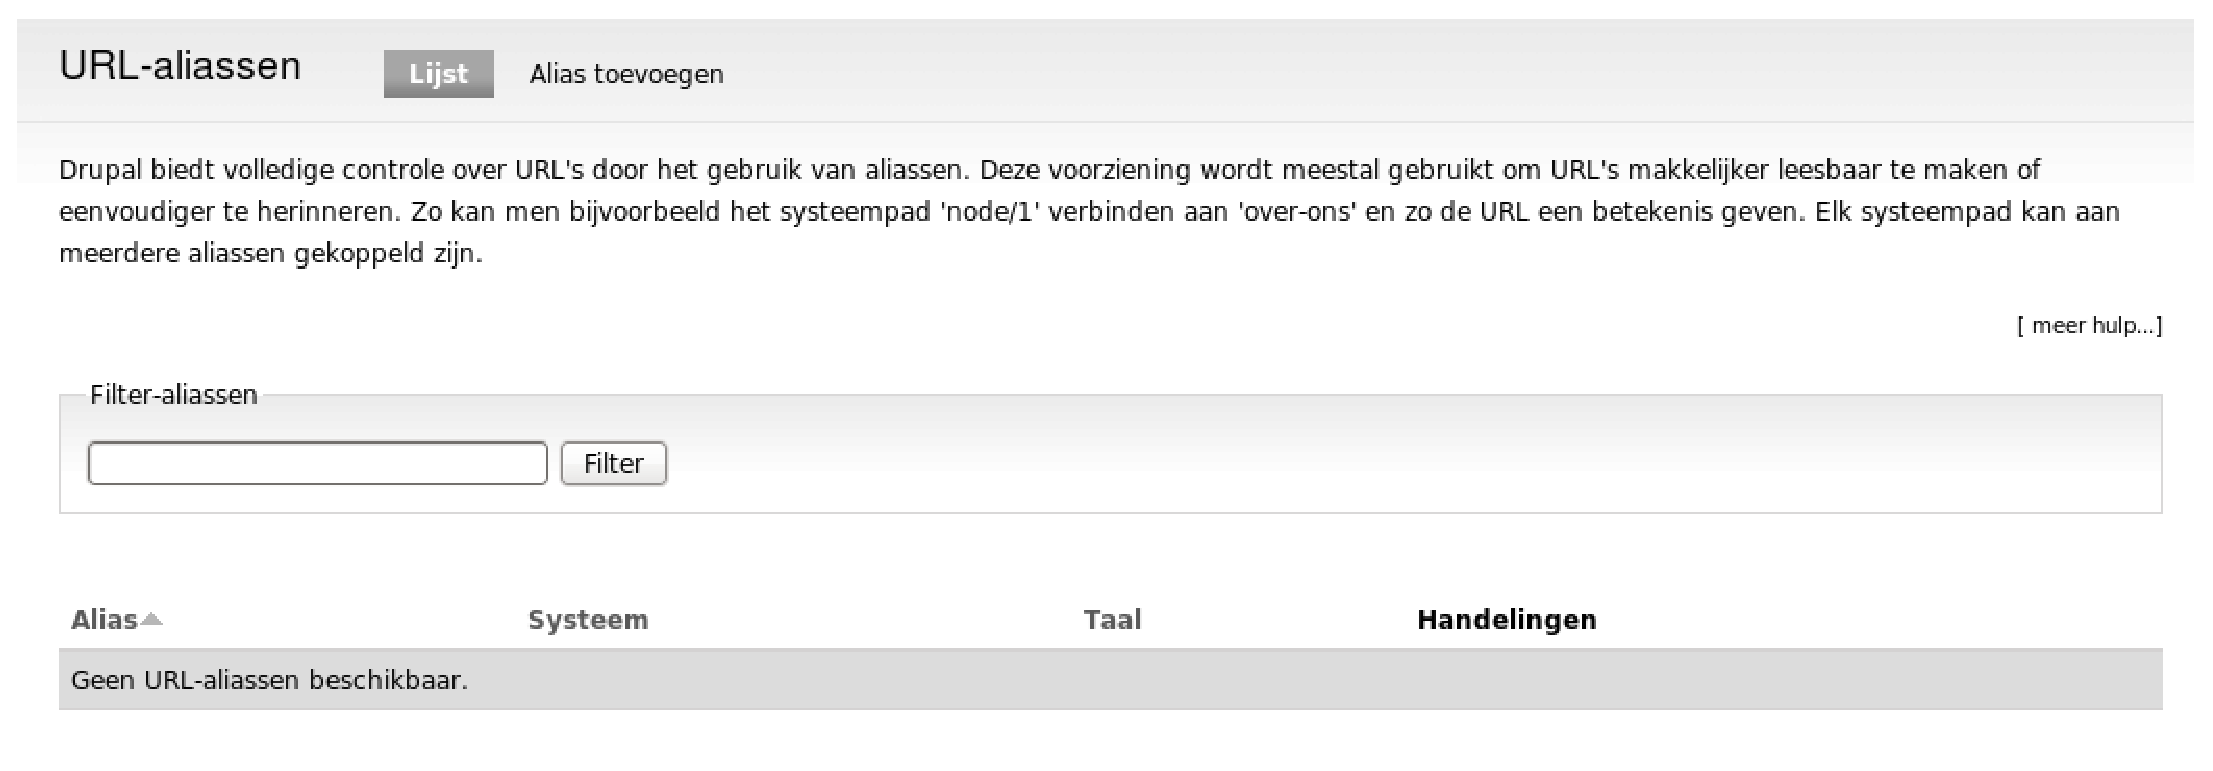
\includegraphics[scale=0.3,angle=0]{url-aliassen-lijst}
   \caption{url-aliassen-lijst.\label{white}}
 \end{figure}
 
\subsection{Alias toevoegen}
 Voer het pad in waarvoor u een alias wenst te cre\"eren, gevolgd door de naam
 van het nieuwe alias.
 \begin{figure}[!h]
    \centering
   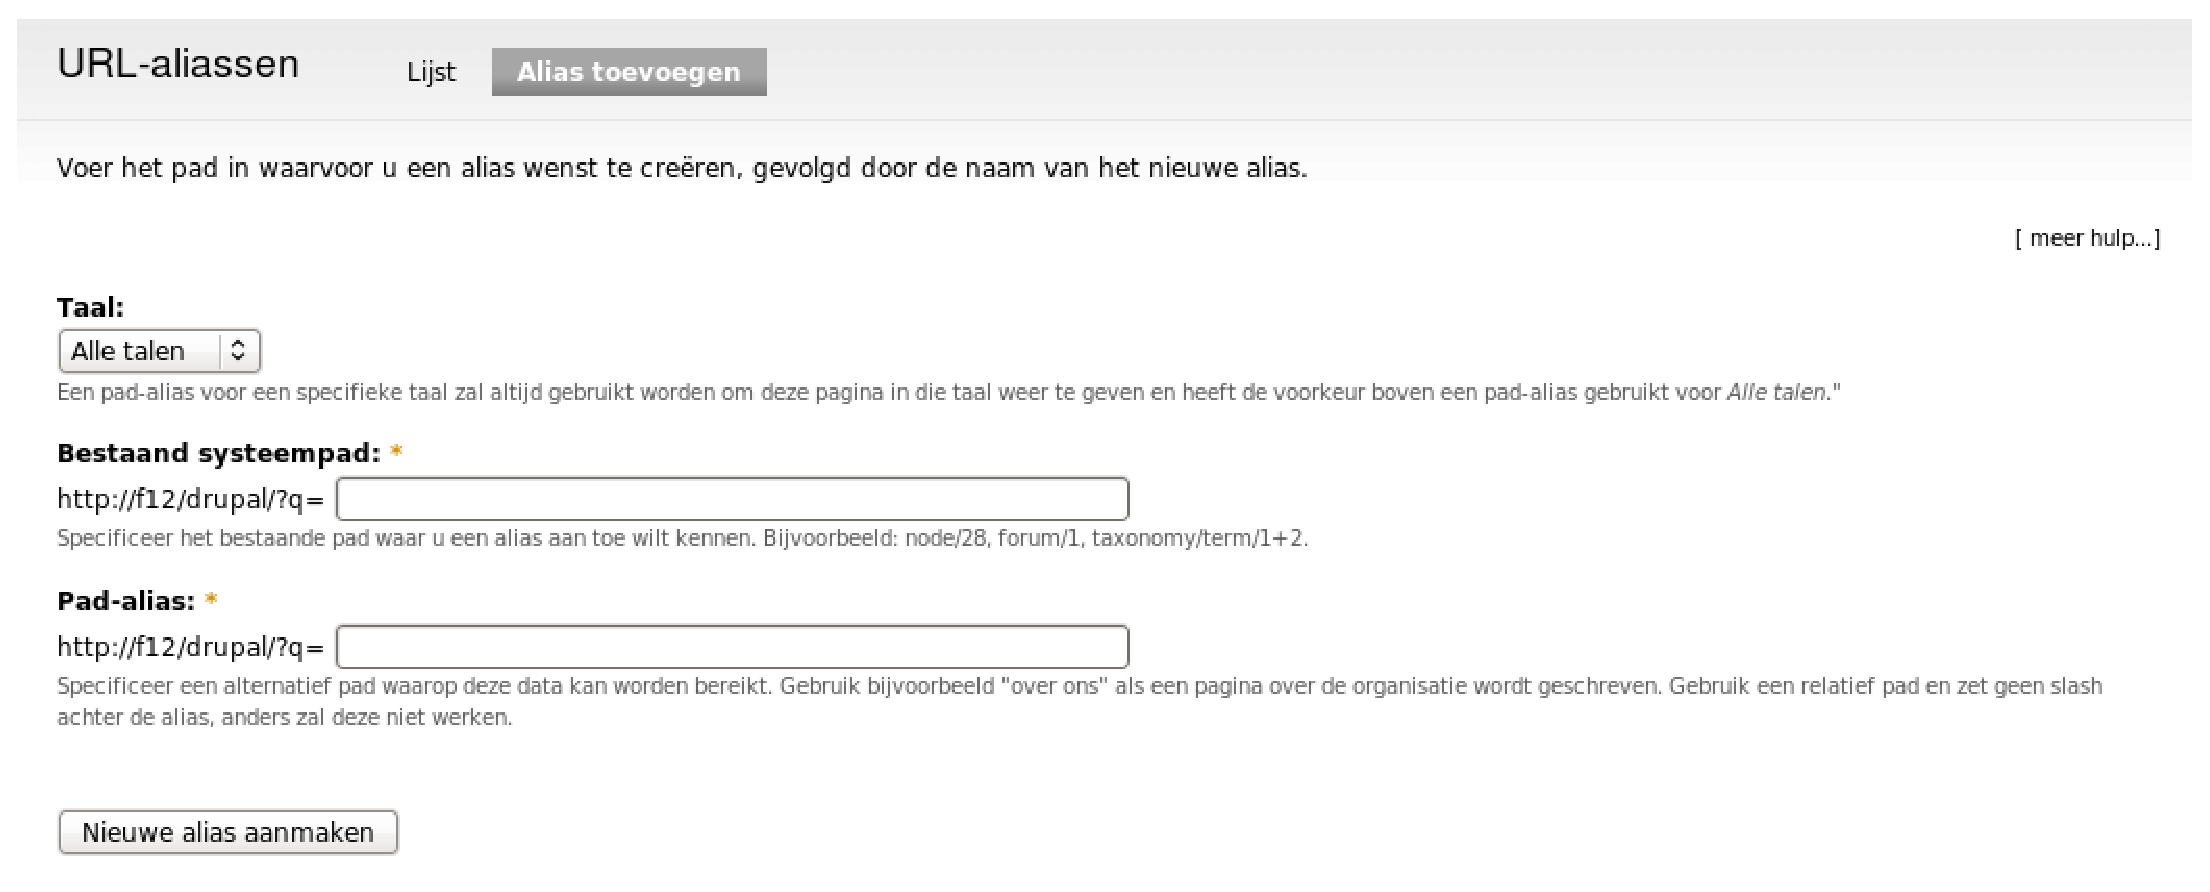
\includegraphics[scale=0.3,angle=0]{url-alias-toevoegen}
   \caption{url-alias-toevoegen.\label{white}}
 \end{figure}
 
\subsection{Path-module} \index{path-module}
Met de Path-module kunt u aliassen voor Drupal-URL's worden opgeven. 
Aliassen verbeteren de leesbaarheid van URL's voor gebruikers en kunnen 
zoekmachines helpen de pagina's effectiever te indexeren. Per pagina mogen meerdere aliassen worden opgegeven.
\\
Enkele voorbeelden van URL-aliassen:
\begin{itemize}
\item user/login $\Rightarrow$ login
\item image/tid/16 $\Rightarrow$ store
\item taxonomy/term/7+19+20+21 $\Rightarrow$ store/products/whirlygigs
\item node/3 $\Rightarrow$ contact
\end{itemize}
Met de Path-module kunnen gebruikers met de juiste toegangsrechten een alias opgeven bij het toevoegen 
of wijzigen van een pagina en het biedt een interface om de aliassen op de site te beheren. 
Twee toegangsrechten die met URL-aliassen samenhangen zijn URL-aliassen beheren en URL-aliassen aanmaken.
\\
De Path-module beschikt ook over de mogelijkheid om volgens eigen specificatie massaal URL-aliassen 
toe te wijzen. Hiermee kunt u eigen uniforme URL's toegepassen, bijvoorbeeld: URL's in een andere taal 
weergeven. Server-toegang tot de Drupal-broncode is nodig om dit soort URL's te realiseren. 
